
\documentclass[a4paper,12pt]{article}

\setlength{\textwidth}{15.0cm}
\setlength{\textheight}{24.0cm}
\setlength{\topmargin}{0cm}
\setlength{\headsep}{0cm}
\setlength{\headheight}{0cm}
\pagestyle{plain}

\usepackage{hyperref}
\hypersetup{
    colorlinks=true,
    linkcolor=blue,
    filecolor=magenta,      
    urlcolor=blue,
    citecolor=blue,
    linktoc=page
}
\usepackage[dvips]{epsfig}
\usepackage{tikz}
\usepackage[english]{babel}
\usepackage{caption}
\captionsetup{font=it}
\usepackage[autostyle, english=american]{csquotes}

\usepackage[
backend=biber,
style=alphabetic,
]{biblatex}

\renewcommand{\bibfont}{\footnotesize}

\usepackage{amsmath,amssymb,amsthm}

\usepackage{comment}
\usepackage{listings}

% \addbibresource{bibliography2.bib} 
\setlength{\parindent}{0pt}

\selectlanguage{english}
\begin{document}

\title{Multigrid for solving complex-valued Helmholtz problems}
\author{Isidoor Pinillo Esquivel}
\date{\today}
\maketitle

\section{Indefinite Helmholtz equation}

\subsection{Discretization}
(a)
\begin{align}
    10                    & \leq \lambda \text{ \#gridpoints} \Leftrightarrow                \\
    10                    & \leq \frac{2\pi}{\sqrt{|\sigma|}} \frac{1}{h^{d}}\Leftrightarrow \\
    \sqrt{|\sigma|} h^{d} & \leq \frac{2 \pi}{10} \approx 0.625.
\end{align}

(b)
\[
    \text{\# gridpoints} = \frac{10 \sqrt{600}}{2 \pi}
    .\]

\subsection{1D model problem}
(a) \\
To proof : $H^{2 h} \neq I_h^{2 h} H^h I_{2 h}^h$.
\begin{align}
    H^{2h} & = H_n = A_n +\sigma {I}_n          \\
    H^{h}  & = H_{2n} = A_{2n} +\sigma {I}_{2n}
\end{align}
Assume that $A_n =I_h^{2 h} A_{2n} I_{2 h}^h= R_{2n} A_{2n} P_n$. By linearity it is  sufficient
to proof:
\begin{align}
    \sigma {I}_n  & \neq \sigma R_{2n} {I}_{2n} P_{n} \Leftrightarrow \\
    {I}_n         & \neq R_{2n} I_{n} \Leftarrow                      \\
    (I_n)_{00} =1 & \neq \frac{3}{4} = (R_{2n} P_{n})_{00}
\end{align}

First equivalence follows from $\sigma \neq 0$. The assumption and the last inequality depends on the definition of
restriction and interpolation. \\
(b) \\
We implemented $f(t) = \delta(t-0.5)$ by concentrating all the mass into the middle element of $f_n$.\\
\begin{figure}[h!]
    \centering
    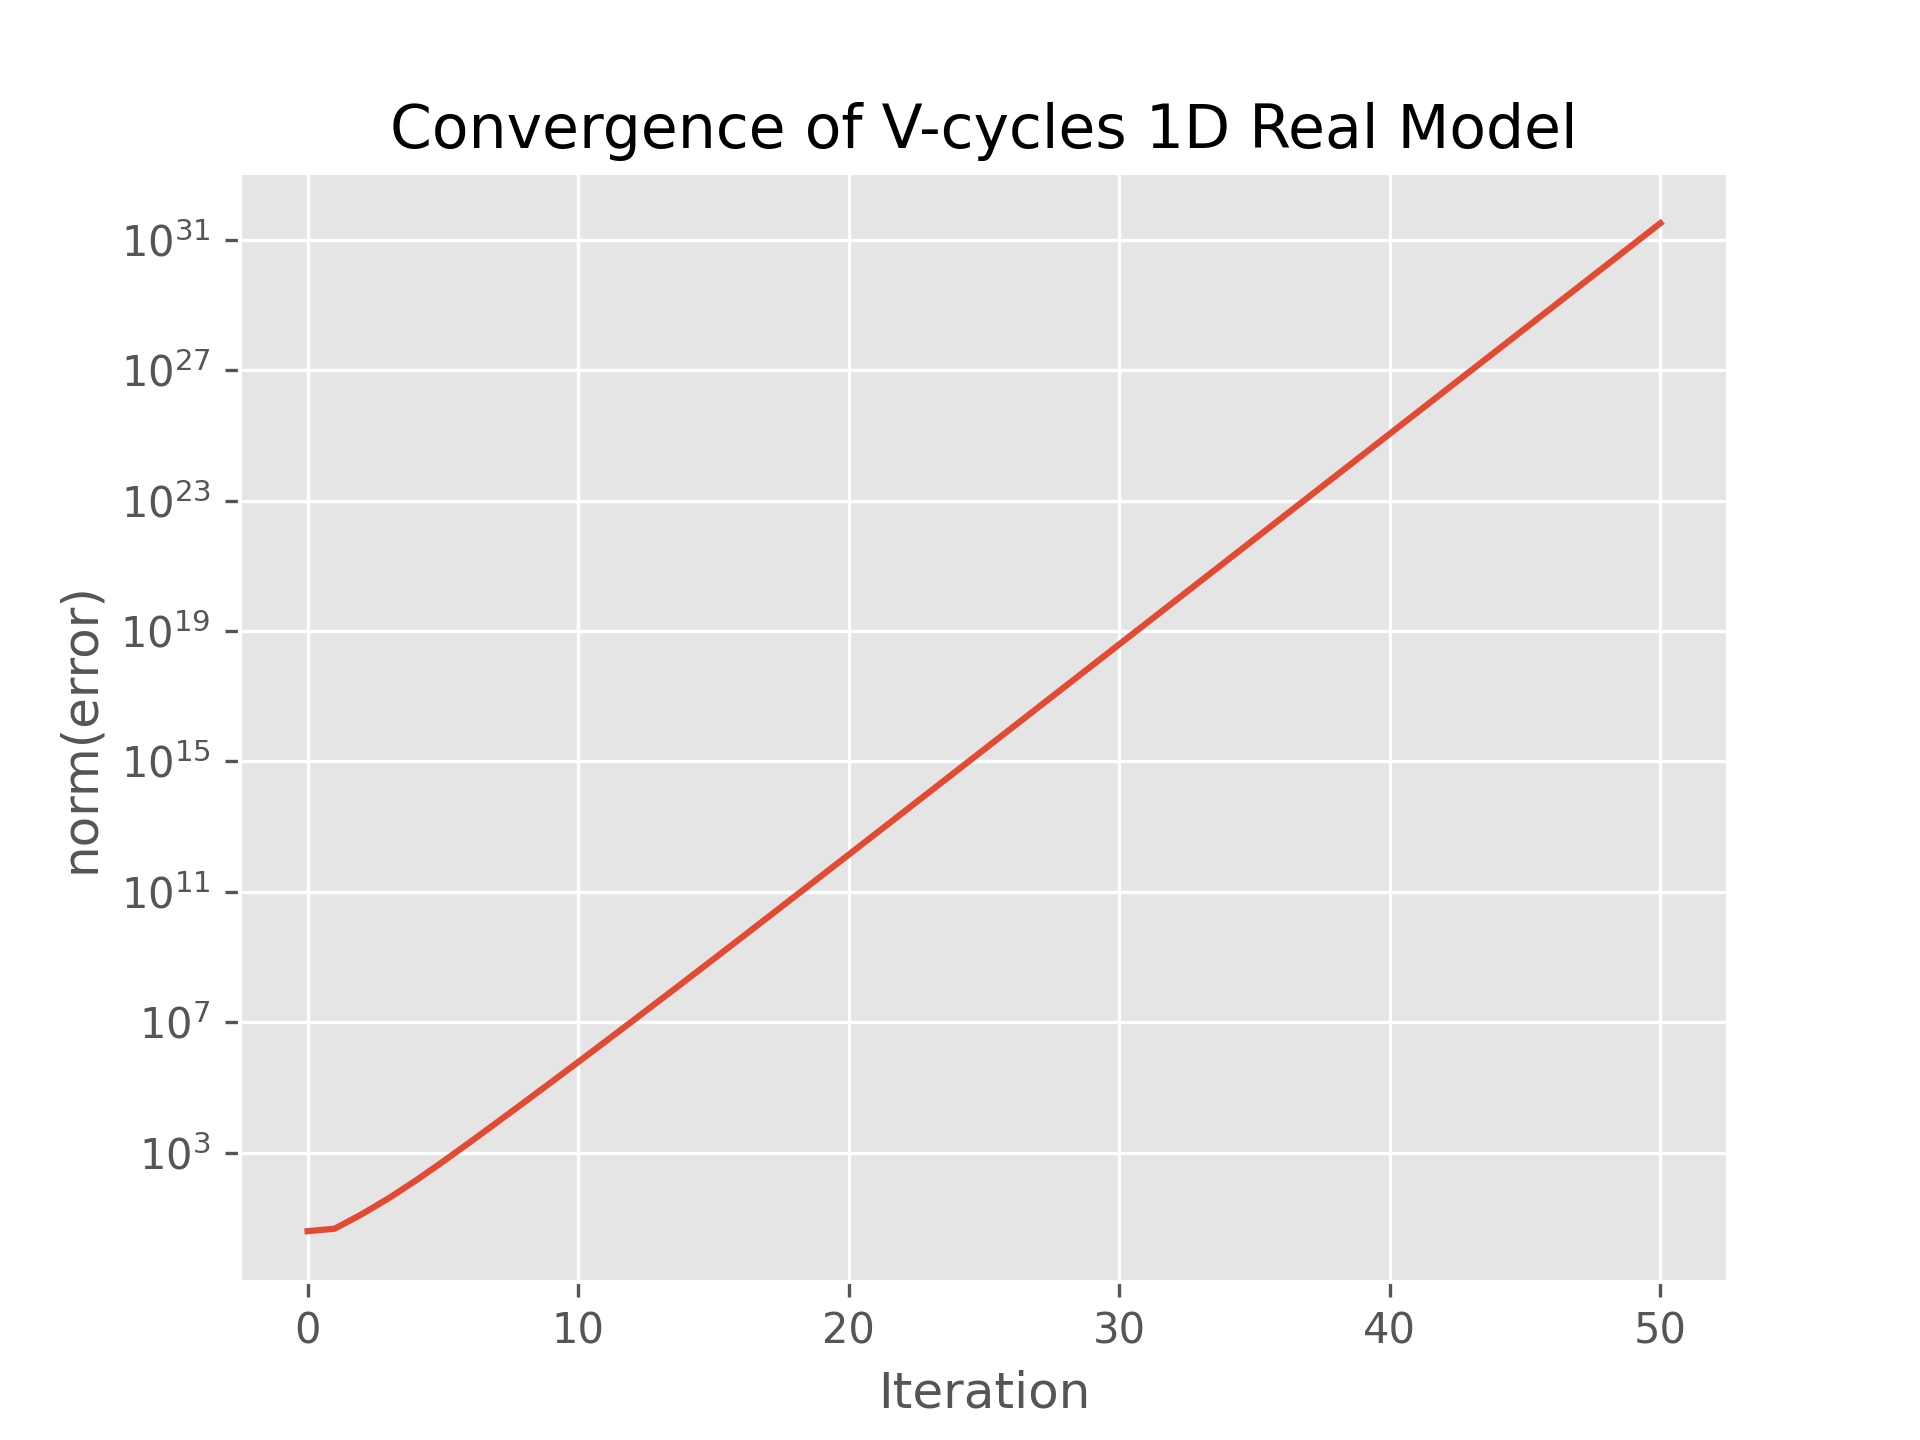
\includegraphics[width=0.8\textwidth]{../code/plts/convergence_1Dreal.png}
    \caption{
        Convergence behavior of the V-cycles for solving
        the discretized Helmholtz equation with $\sigma = -600, n = 64$.
        The V-cycles seems to diverge,
        suggesting challenges in solving the Helmholtz problem using this approach.
    }

    \label{fig:1Dreal}
\end{figure}


(c) \\
The eigenvalues and eigenvectors can be derived from the Poisson problem ($\sigma=0$) because
\begin{align}
    Av            & = \lambda v \Rightarrow \\
    (A+\sigma I)v & = Av + \sigma v         \\
                  & = (\lambda+\sigma)v
\end{align}
i.e. eigenvectors stay the same and eigenvalues get shifted by $\sigma$. \\

(d) \\
$\sigma = 0$ is the boundary where $H$ goes from indefinite to definite.
\begin{figure}[h!]
    \centering
    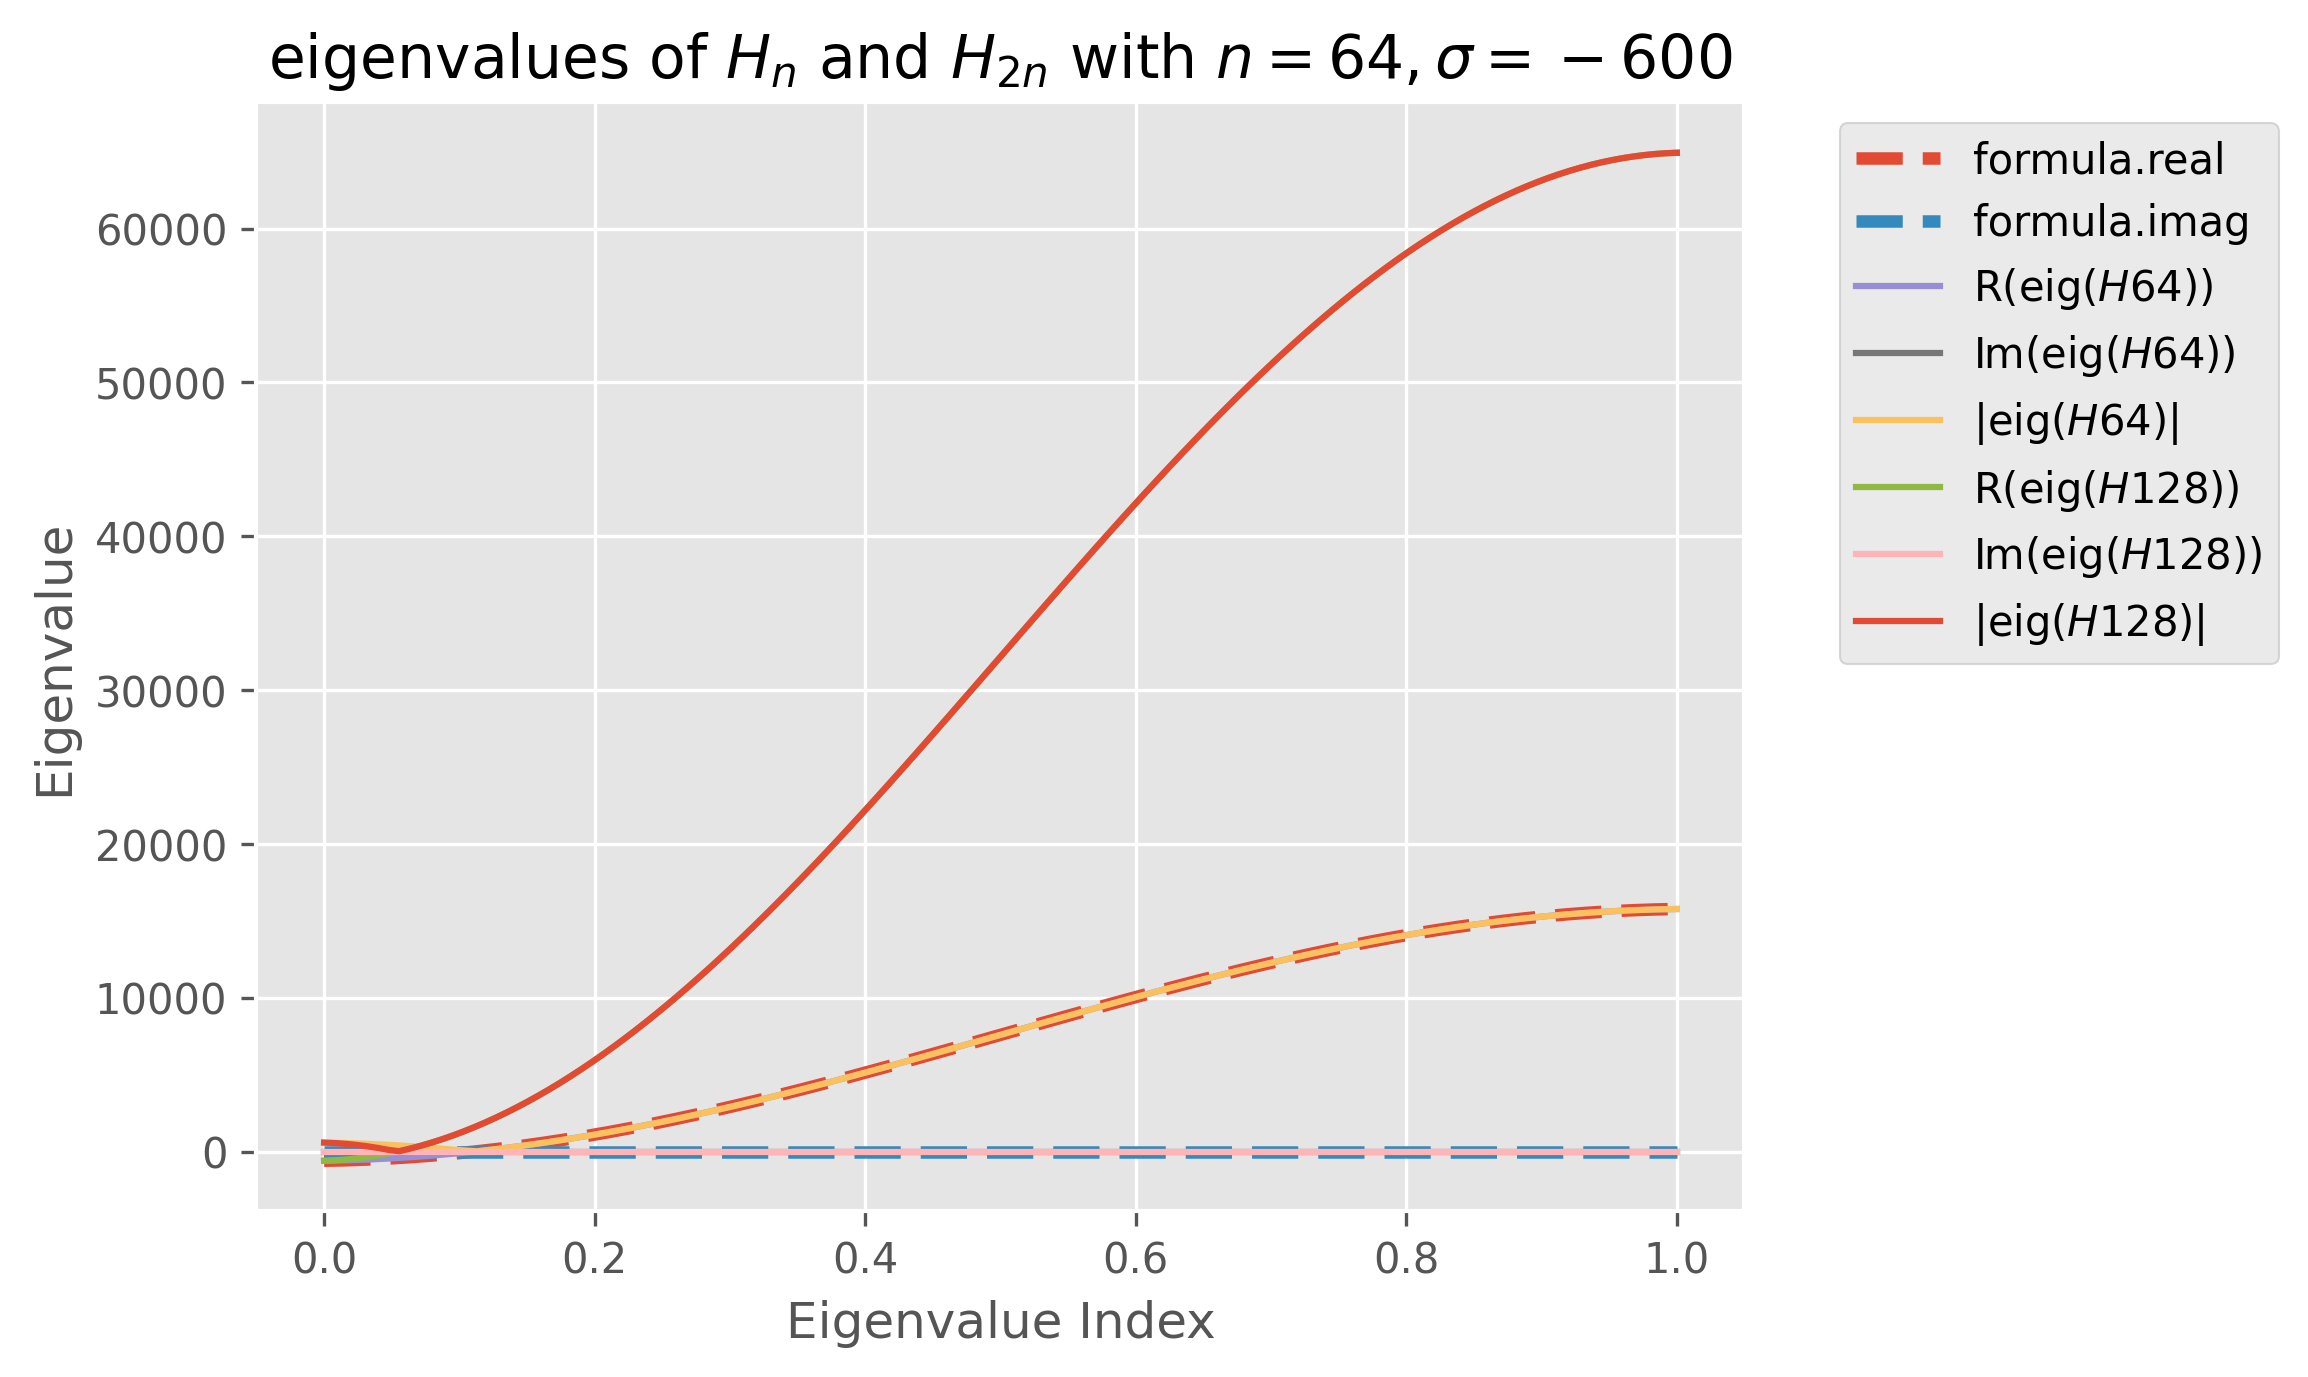
\includegraphics[width=0.8\textwidth]{../code/plts/eigenvalues_1Dreal.png}
    \caption{We sorted the eigenvalues and scaled the x-axis to make it easier to compare eigenvalues.
        Note that $H_{2n}$ has twice the amount of eigenvalues then $H_{n}$.}
    \label{fig:eigen 1D real}
\end{figure}


\subsection{LFA analysis of the $\omega$-Jacobi smoother}
(a) \\
For grid points without a neighboring boundary point there
$H$ acts like following stencil:
\[
    H_n = n^{2} [ -1 \quad 2+ \frac{\sigma}{n^{2}}  \quad -1]
    .\]

So $R_{\omega}$ works element wise the following way on the error:
\begin{equation}
    e_{j}^{m+1} = (1-\omega) e_{j} ^{m} + \frac{\omega n^{2}}{2 n^{2} + \sigma} (e_{j-1} ^{m} + e_{j+1}^{m})
    .
\end{equation}
The LFA analysis for the Helmholtz equation is very similar to the analysis for the Poisson equation.
Doing the LFA subsitution $e_j^{(m)}=\mathcal{A}(m) e^{i j \theta}$:

\begin{align}
    A(m+1)    & = A(m) \left( 1-\omega + \frac{\omega n^{2}}{2 n^{2} + \sigma} (e^{-i\theta} + e^{i\theta}) \right) \\
              & = A(m) \left( 1-\omega + 2 \cos(\theta) \frac{\omega n^{2}}{2 n^{2} + \sigma}   \right) \Rightarrow \\
    G(\theta) & = \left( 1-\omega + 2 \cos(\theta) \frac{\omega n^{2}}{2 n^{2} + \sigma}   \right)
\end{align}

Note that we haven't used that $\sigma$ is real. \\
(b) \\
$\sigma = 0$ reduces back to the LFA we did for the Poisson equation.
$\theta \approx 0 \Rightarrow \cos(\theta)
    \approx 1 + O \left(\frac{1}{n^{2}}\right) \Rightarrow G(\theta) \approx 1 - O \left(\frac{1}{n^{2}}\right)$
so smooth modes are preserved for big $n$. For $\sigma<0$ $G(\theta)$ becomes slightly bigger than $1$
i.e. smooth modes get amplified.\\
\begin{figure}[h!]
    \centering
    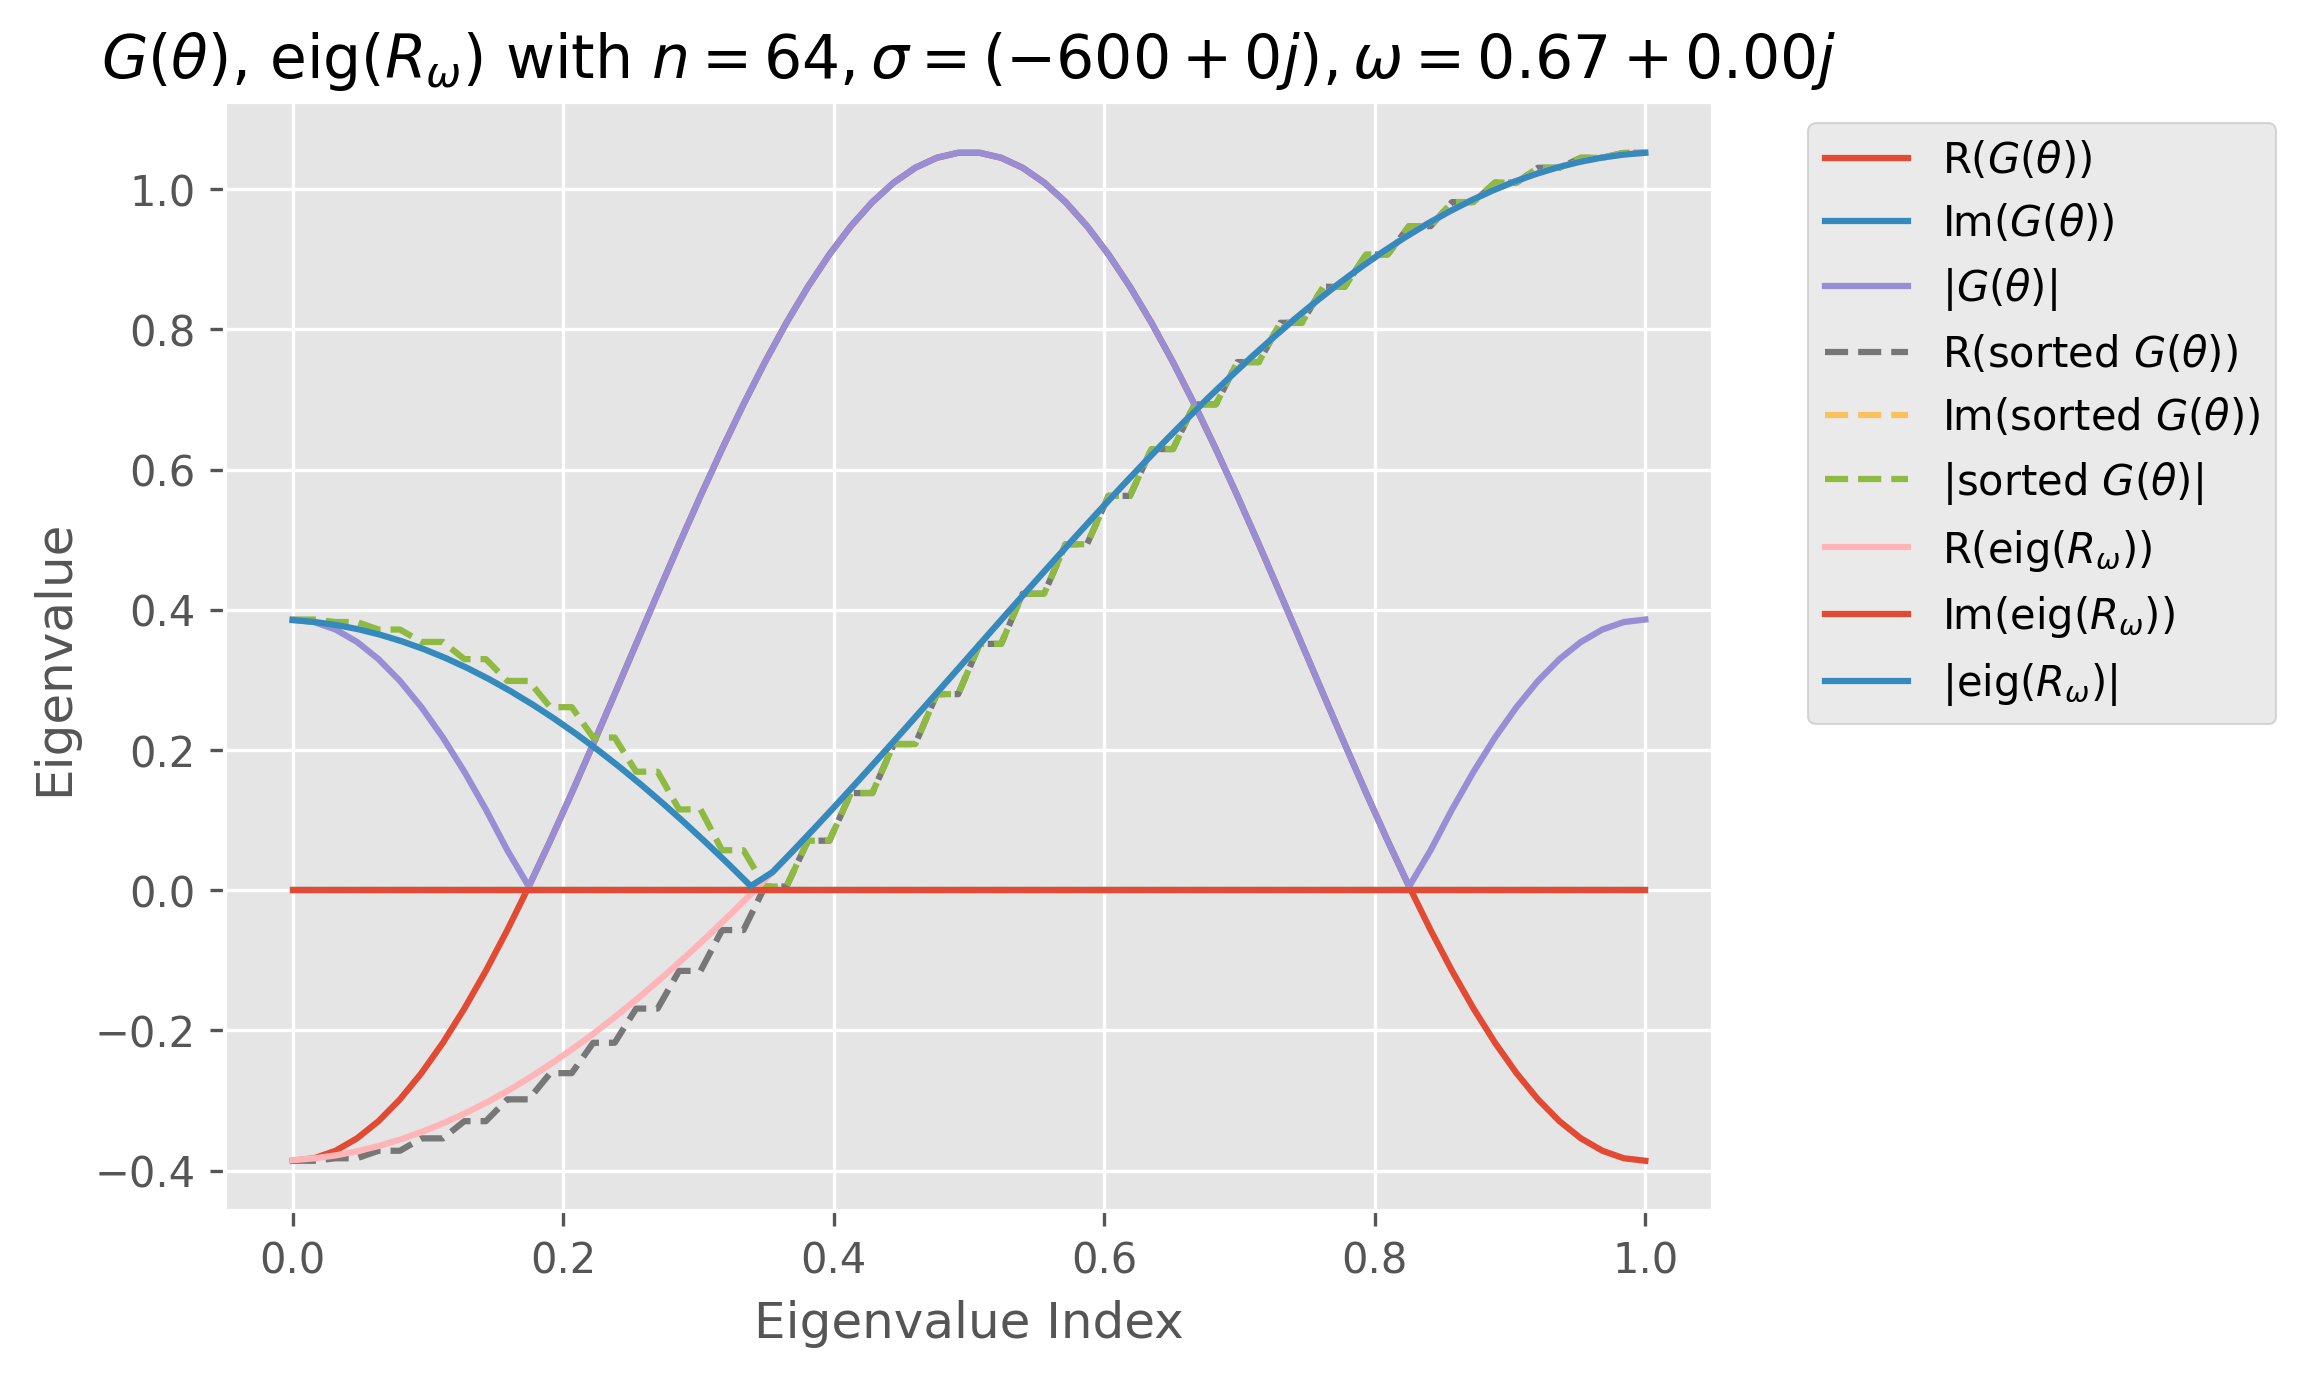
\includegraphics[width=0.8\textwidth]{../code/plts/eigenvalues_1DrealG.png}
    \caption{We sorted the eigenvalues and scaled the x-axis to make it easier to compare eigenvalues.}
    \label{fig:eig real1D G}
\end{figure}

(d)\\
Maximum of $G(\theta)$ is achieved at $\theta =0$ because $G(\theta)$ is just
an increasing function of $\cos(\theta)$ then try the minima and maxima of $cos$.
This means that
$\rho = |1-\omega + 2 \frac{\omega n^{2}}{2 n^{2} + \sigma}|  \approx 1.05 $
which suggests that in the worst case the smoother my amplify error with a factor of $1.05$.


\subsection{Spectral analysis of the two-grid correction scheme}
(a) \\
It is easily seen that
\begin{equation}
    R_{2n} =  c S_{2n} (3I_{2n} -A_{2n}).
\end{equation}
with $c \in \mathbb{R}_{0}$, $S_{2n}: \mathbb{R}^{2n-1} \rightarrow \mathbb{R}^{n-1}: (v_{j})_{j \leq 2n-2}
    \rightarrow (v_{2j+1})_{j \leq n-2}$  subsampling uneven components.
Using that $S_{2n}w_{k}^{2n} = w_{k}^{n}$ if $k<n$ it is easily seen that:
\begin{align}
    R_{2n} w_{k}^{2n} & = cS_{2n}(3I_{2n}- A_{2n}) w_{k}^{2n}         \\
                      & = c(3- \lambda_{k}(A_{2n})) S_{2n} w_{k}^{2n} \\
                      & = a(n,k) w_{k}^{n} .
\end{align}
Good interpolation has by definition low reconstruction error.
In our case $P_{n}$ is linear interpolation, reconstuction error for lagrange interpolation can be bounded
using Taylors theorem.
\begin{equation}
    P_{n} S_{2n} v_{2n}  \approx c v_{2n}.
\end{equation}
For $w_{k}^{2n}$ smooth and combining with previous argument we have:
\begin{equation}
    P_{n} R_{2n} w_{2n}  \approx c_{1} w_{2n}.
\end{equation}
To check the normalizing constant try $v_{2n} = 1 \Rightarrow c_{1} =1$. \\
Now doing spectral analysis of TG is straight forward:
\begin{align}
    TG w_{k}^{2n} & = (I_{n} - P_{n} H_{n}^{-1} R_{2n} H_{2n}) w_{k}^{2n}                                 \\
                  & =  w_{k}^{2n} - P_{n} H_{n}^{-1} R_{2n} \lambda_{k}(H_{2n}) w_{k}^{2n}                \\
                  & =  w_{k}^{2n} - P_{n} H_{n}^{-1}  a(n,k) w_{k}^{n} \lambda_{k}(H_{2n})                \\
                  & =  w_{k}^{2n} - P_{n}  a(n,k) w_{k}^{n} \lambda_{k}(H_{n}^{-1})  \lambda_{k}(H_{2n})  \\
                  & =  w_{k}^{2n} - P_{n}  R_{2n} w_{k}^{2n} \lambda_{k}(H_{n}^{-1})  \lambda_{k}(H_{2n}) \\
                  & \approx  w_{k}^{2n} -  w_{k}^{2n} \lambda_{k}(H_{n}^{-1})  \lambda_{k}(H_{2n})        \\
                  & \approx  w_{k}^{2n} (1-   \lambda_{k}(H_{n}^{-1})  \lambda_{k}(H_{2n})).
\end{align}

(b) \\
We already analytically derived the eigenvalues for $H_{n}$.
\begin{figure}[h!]
    \centering
    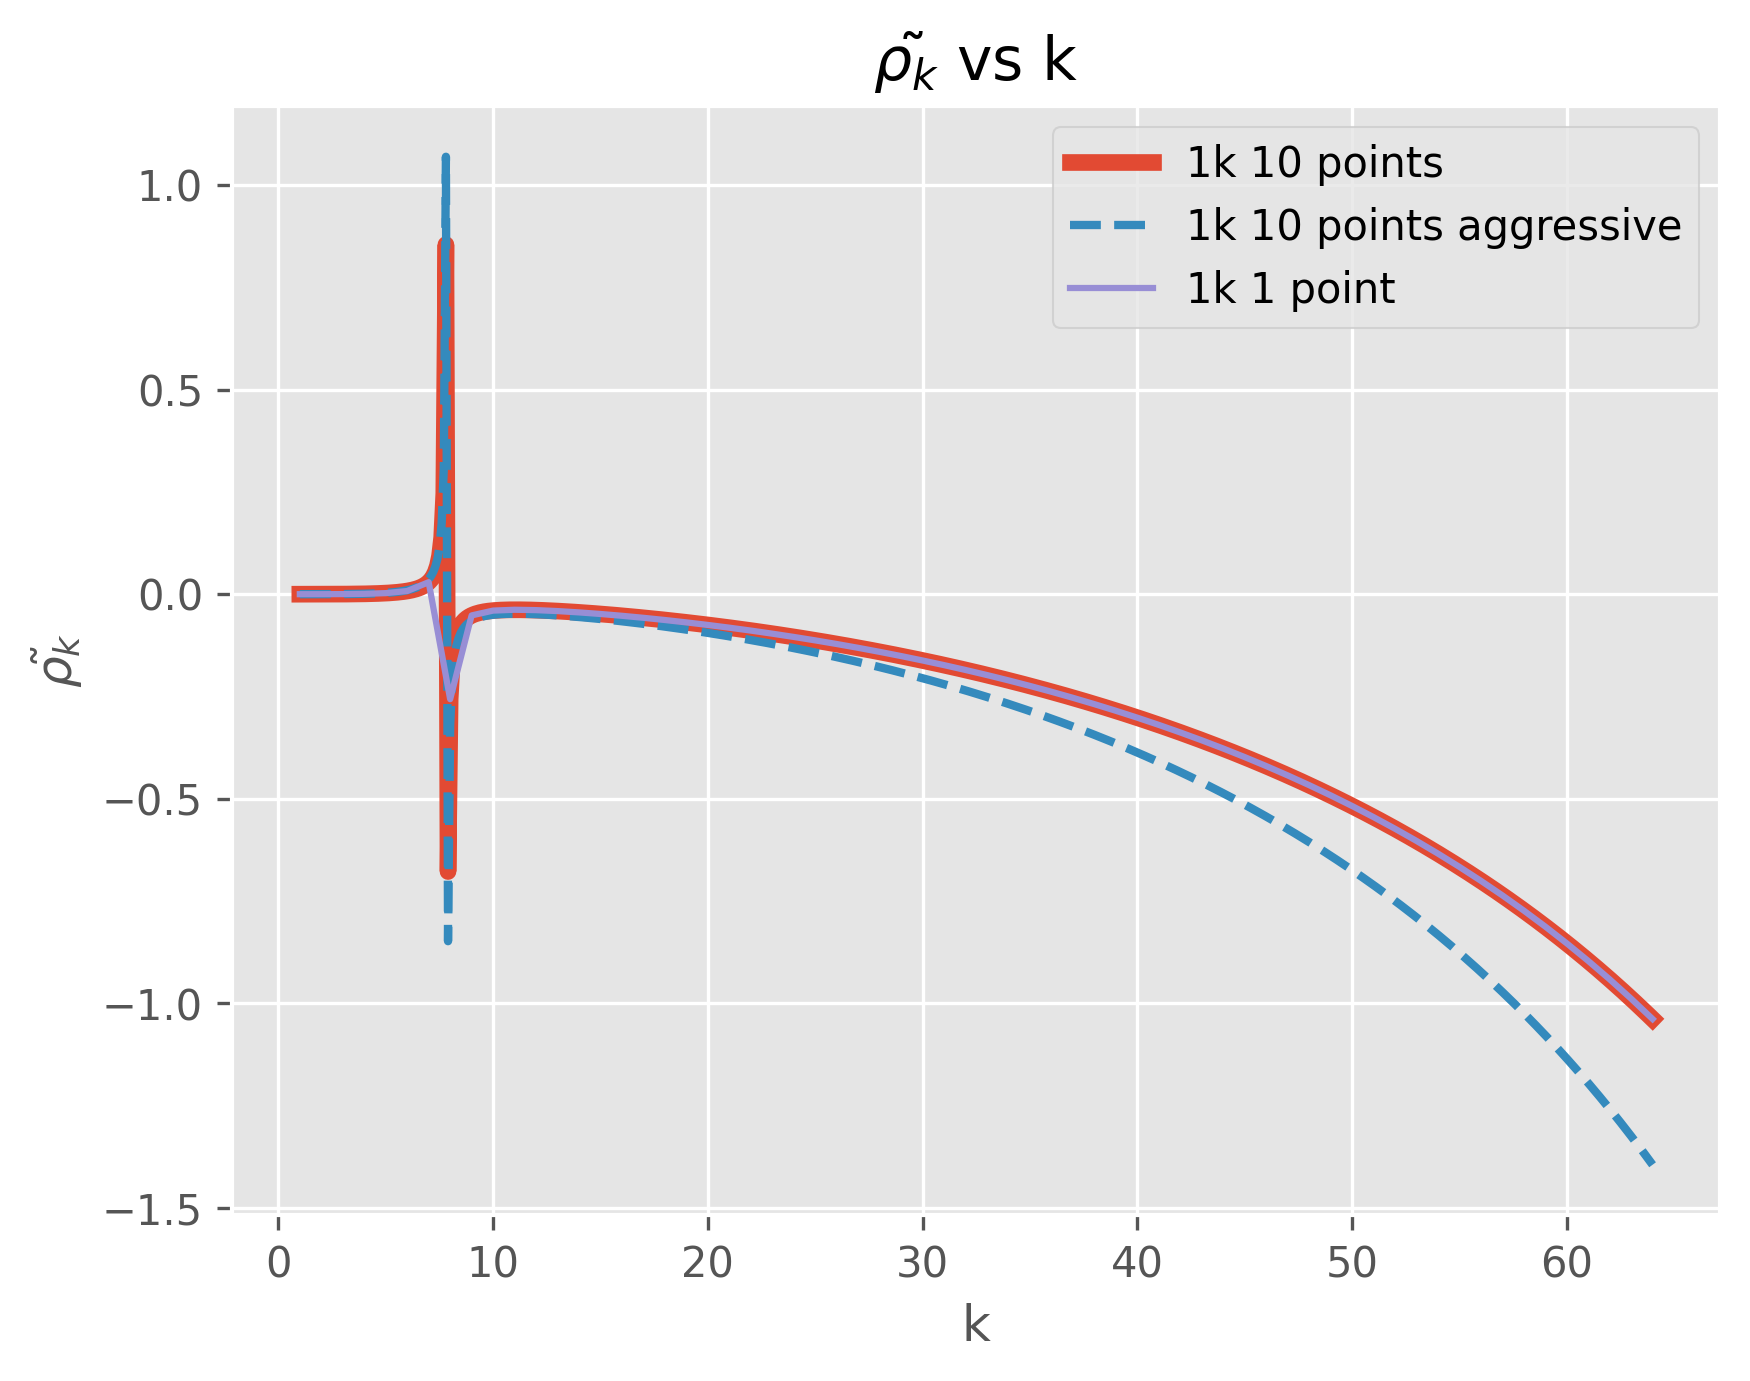
\includegraphics[width=0.8\textwidth]{../code/plts/rho_k_1DrealG.png}
    \caption{The spike represents the bad behavior of TG for the Helmholtz problem.}
    \label{fig:rho_k vs k real}
\end{figure}

Sometimes a specific smooth eigenmode doesn't get dampend or even amplified by a TG iteration which is undesired. \\
(c)\\
See Figure \ref{fig:eigen 1D real}.  Obviously when the signs of $\lambda_{k}(H_{n}^{-1})$  and $\lambda_{k}(H_{2n})$
leads to $\tilde{\rho_k}$ which explains the spike. For $n = 64$ and $\sigma= -600$ the
index closest to the sign change is $k = 6$. No, the smoother leaves smooth modes almost unchanged.\\

Combining the poor predicted performance of the smoother and TG-iteration it is not
surprising that the V-cycles diverged.


\section{Solving the complex-valued Helmholtz problem using Multigrid}


\subsection{1D model problem}
(a) \\
For $\sigma = -600-300j, n = 64$ the problem does converges.
\begin{figure}[h!]
    \centering
    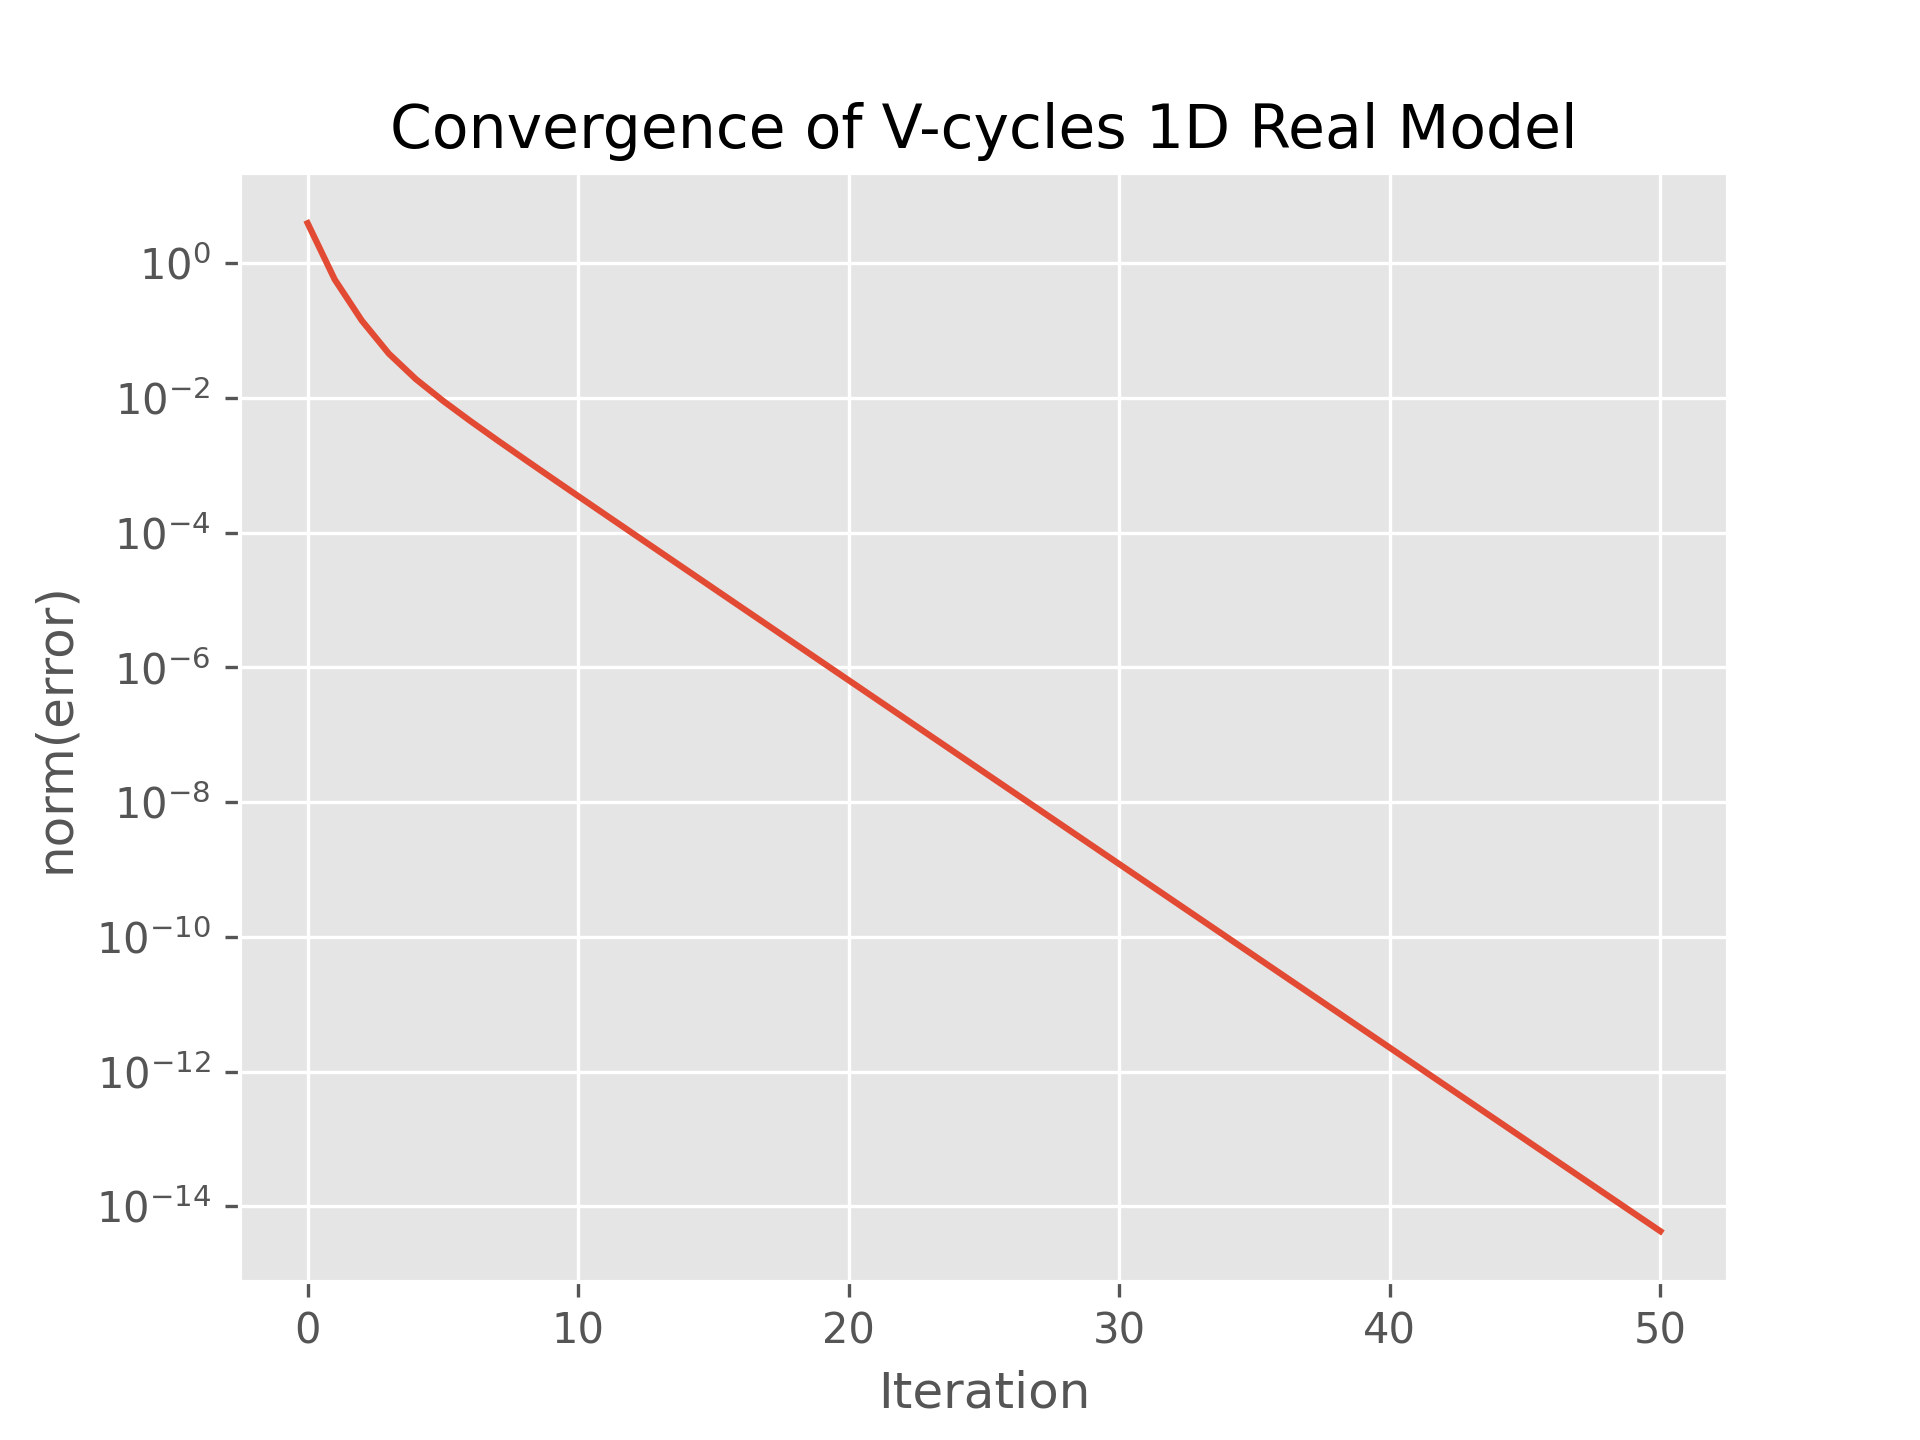
\includegraphics[width=0.8\textwidth]{../code/plts/convergence_1Dcomplex.png}
    \caption{
        Convergence behavior of the V-cycles for solving
        the discretized Helmholtz equation with $\sigma = -600-300j, n = 64$.
    }
    \label{fig:1Dcomplex}
\end{figure}

(b)\\
For a point source it was not be obvious so we used $f_{n} = w_{10}^{n}$ but the solution
for the complex shifted problem is very similar.

\begin{figure}[h!]
    \centering
    \hspace*{-1.55cm}
    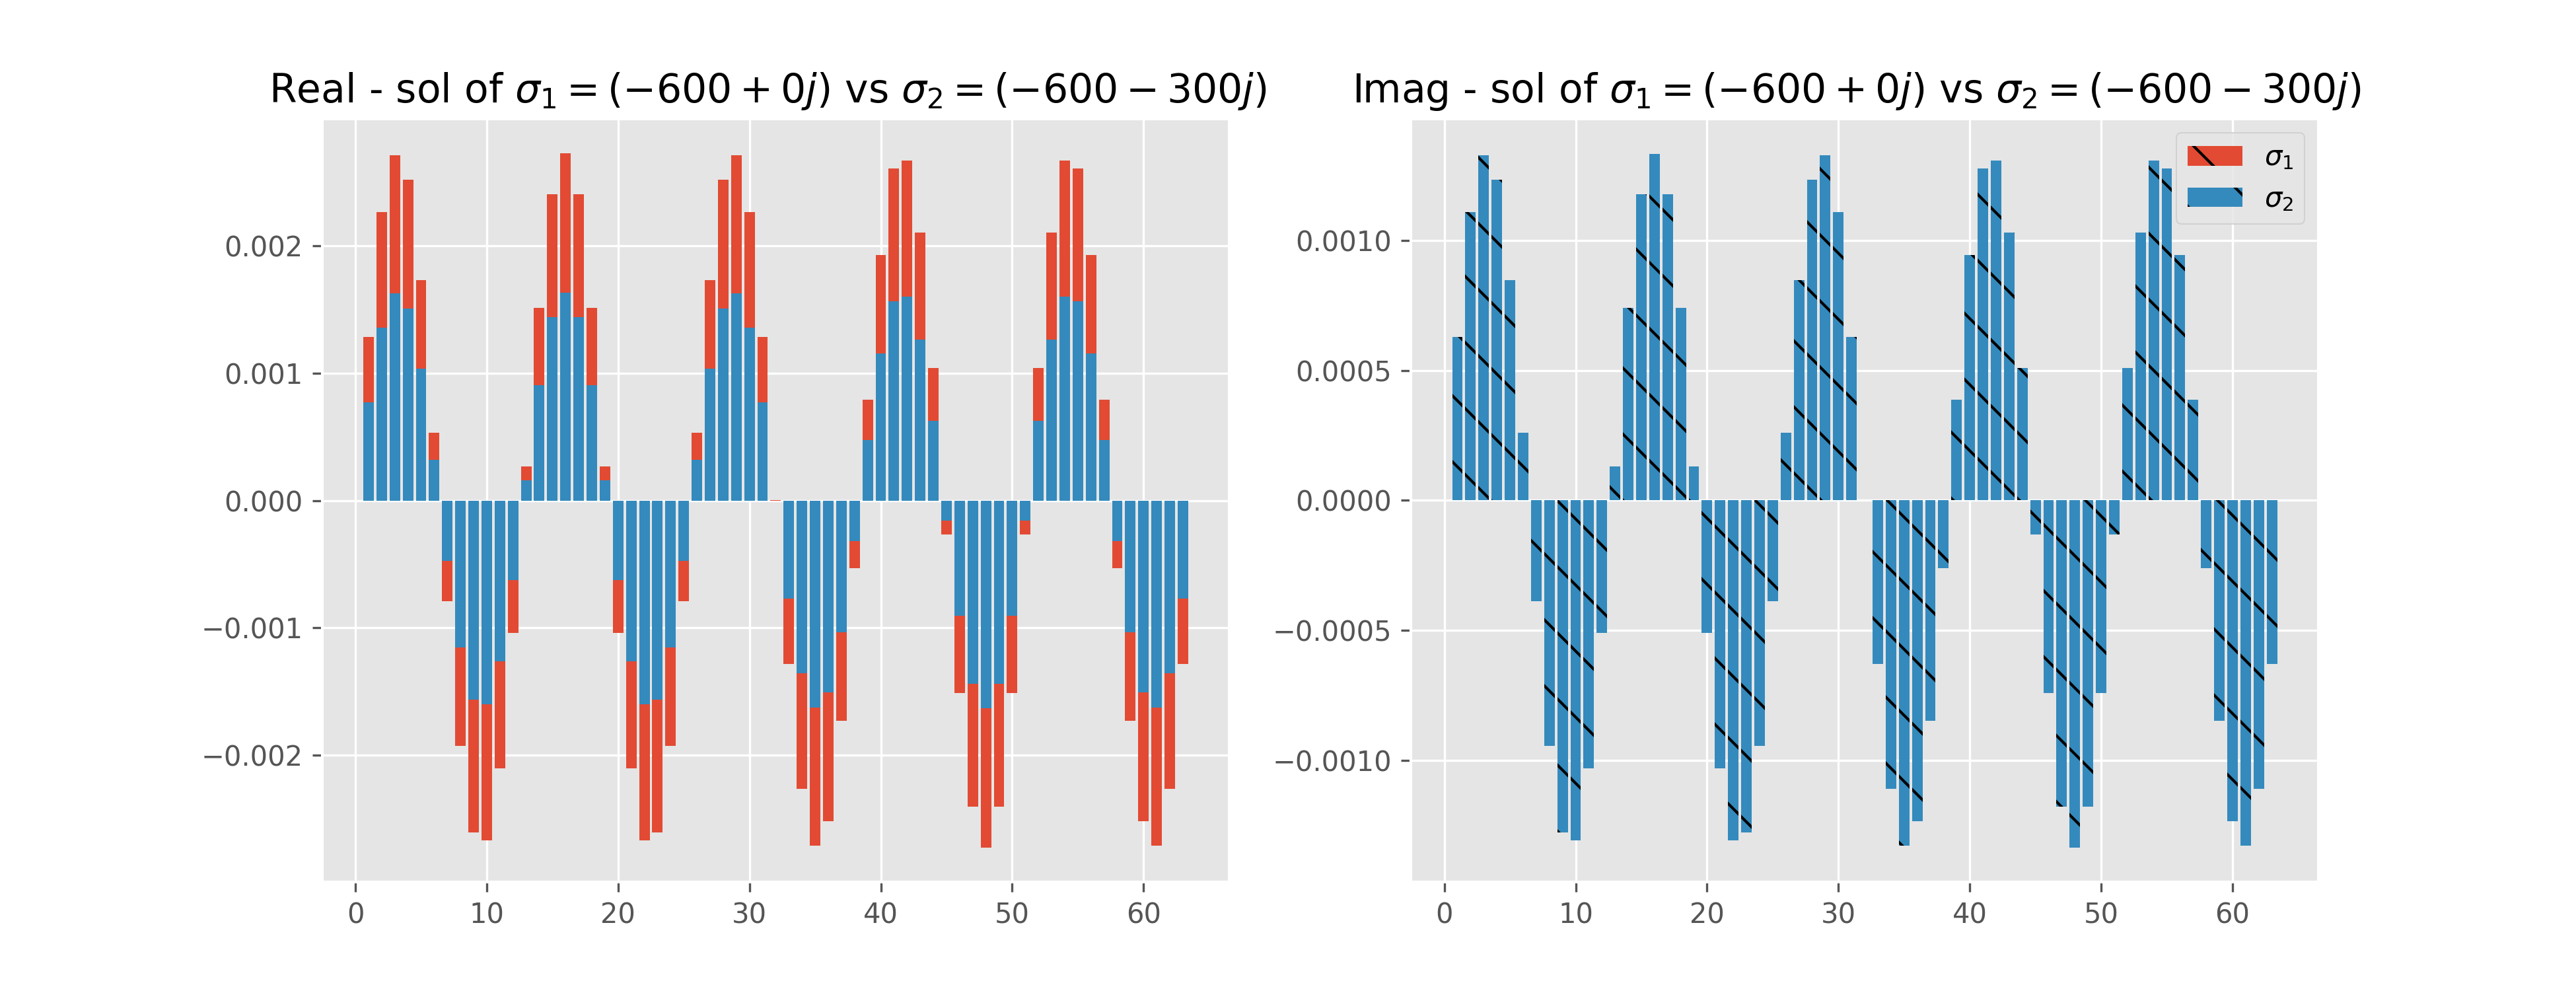
\includegraphics[width=1.2\textwidth]{../code/plts/exact_1Dcomplex.png}
    \caption{Exact solutions for $n=64,  f_{n}= w_{10}^{n}$ comparing $\sigma_{1} = -600$ and $\sigma_{2} =-600-300j$.}
    \label{fig: exact 1D complex}
\end{figure}

(c) \\
We already analytically derived the eigenvalues for $H_{n}$. Again the spectrum get shifted by the complex shift.

\begin{figure}[h!]
    \centering
    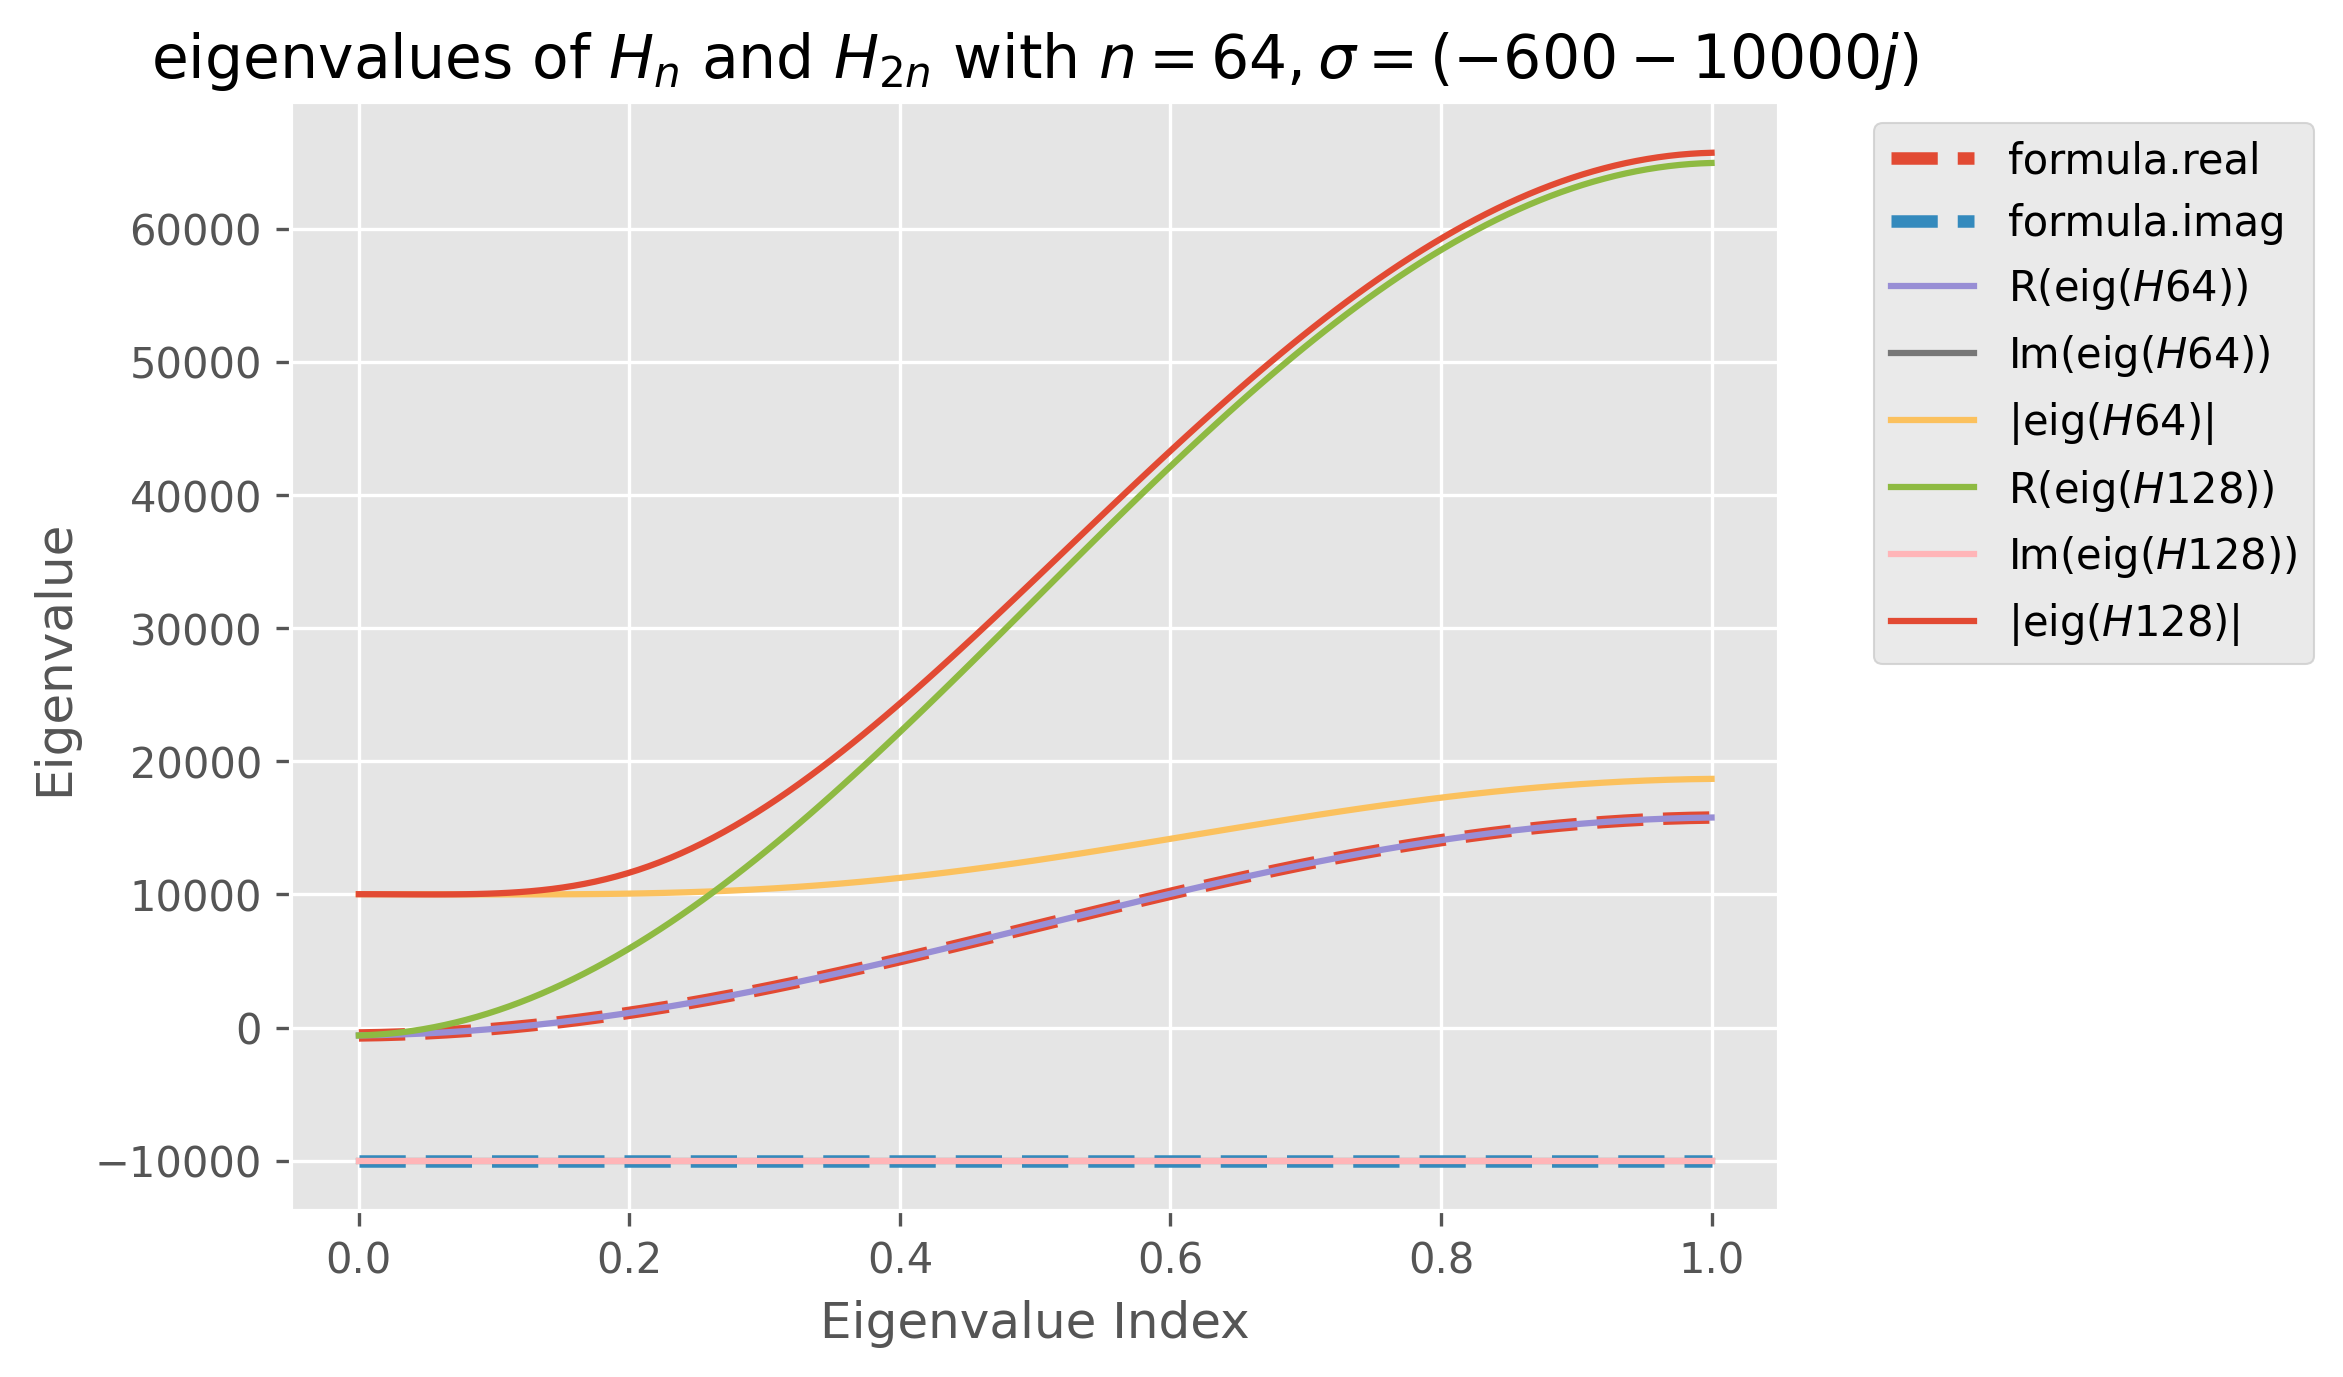
\includegraphics[width=0.8\textwidth]{../code/plts/eigenvalues_1Dcomplex.png}
    \caption{We sorted the eigenvalues and scaled the x-axis to make it easier to compare eigenvalues.
        Note that $H_{2n}$ has twice the amount of eigenvalues then $H_{n}$.}
    \label{fig: eigen complex 1D}
\end{figure}


\subsection{LFA analysis of the $\omega$-Jacobi smoother}
(a) \\
Already answered in previous question. $\rho$ is still $|G(0)|$ almost the same reasoning.
\begin{equation}
    |G(\theta)| = |a + b \cos(\theta) + c \cos(\theta)i|
\end{equation}
with $a,b \in \mathbb{R}^{+}$ and $c \in  \mathbb{R}$ still gets optimized when $\cos\left(\theta\right)$
gets optimized.

(b) \\
\begin{figure}[h!]
    \centering
    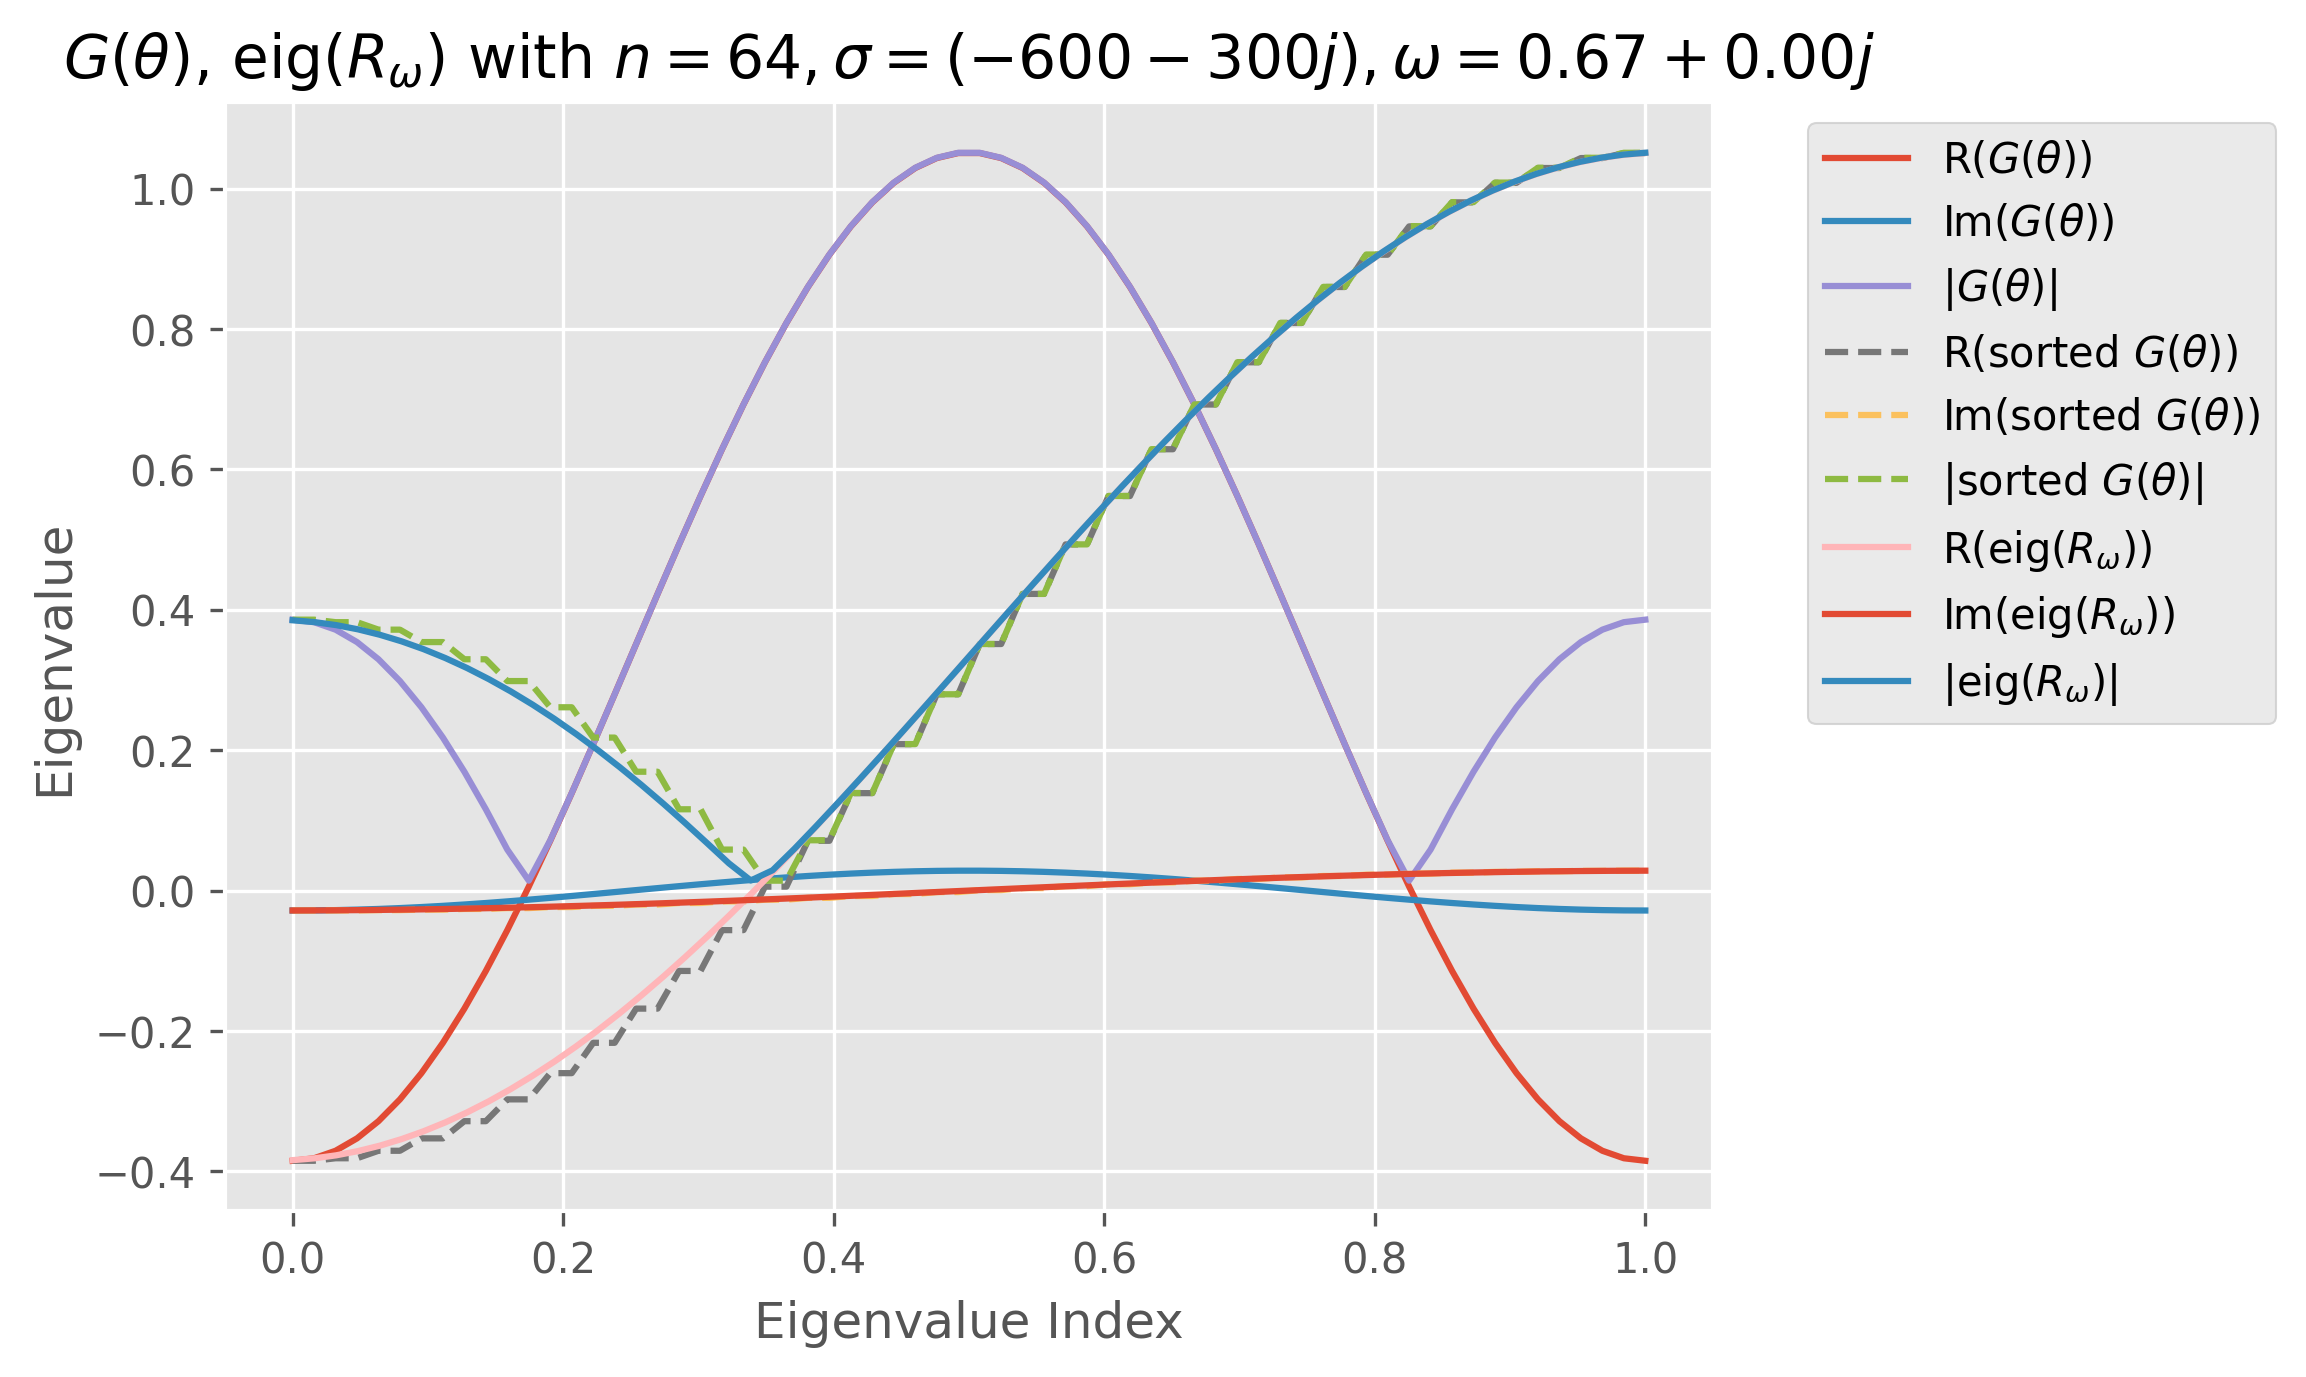
\includegraphics[width=0.8\textwidth]{../code/plts/eigenvalues_1DcomplexG.png}
    \caption{We sorted the eigenvalues and scaled the x-axis to make it easier to compare eigenvalues.}
    \label{fig:eigen complex G 1D}
\end{figure}
Not much is changed compared the real case. \\
(c) \\
It is either $|G(\pi)|$ or $|G(\frac{\pi}{2})|$
see main.ipynb. For $\omega = 2/3$ they are roughly equal with $\mu = \frac{1}{3}$.\\
(d) \\
Eyeballing Figure \ref{fig:rho omega 1D complex}, $\omega \approx 0.65$ is good.
\begin{figure}[h!]
    \centering
    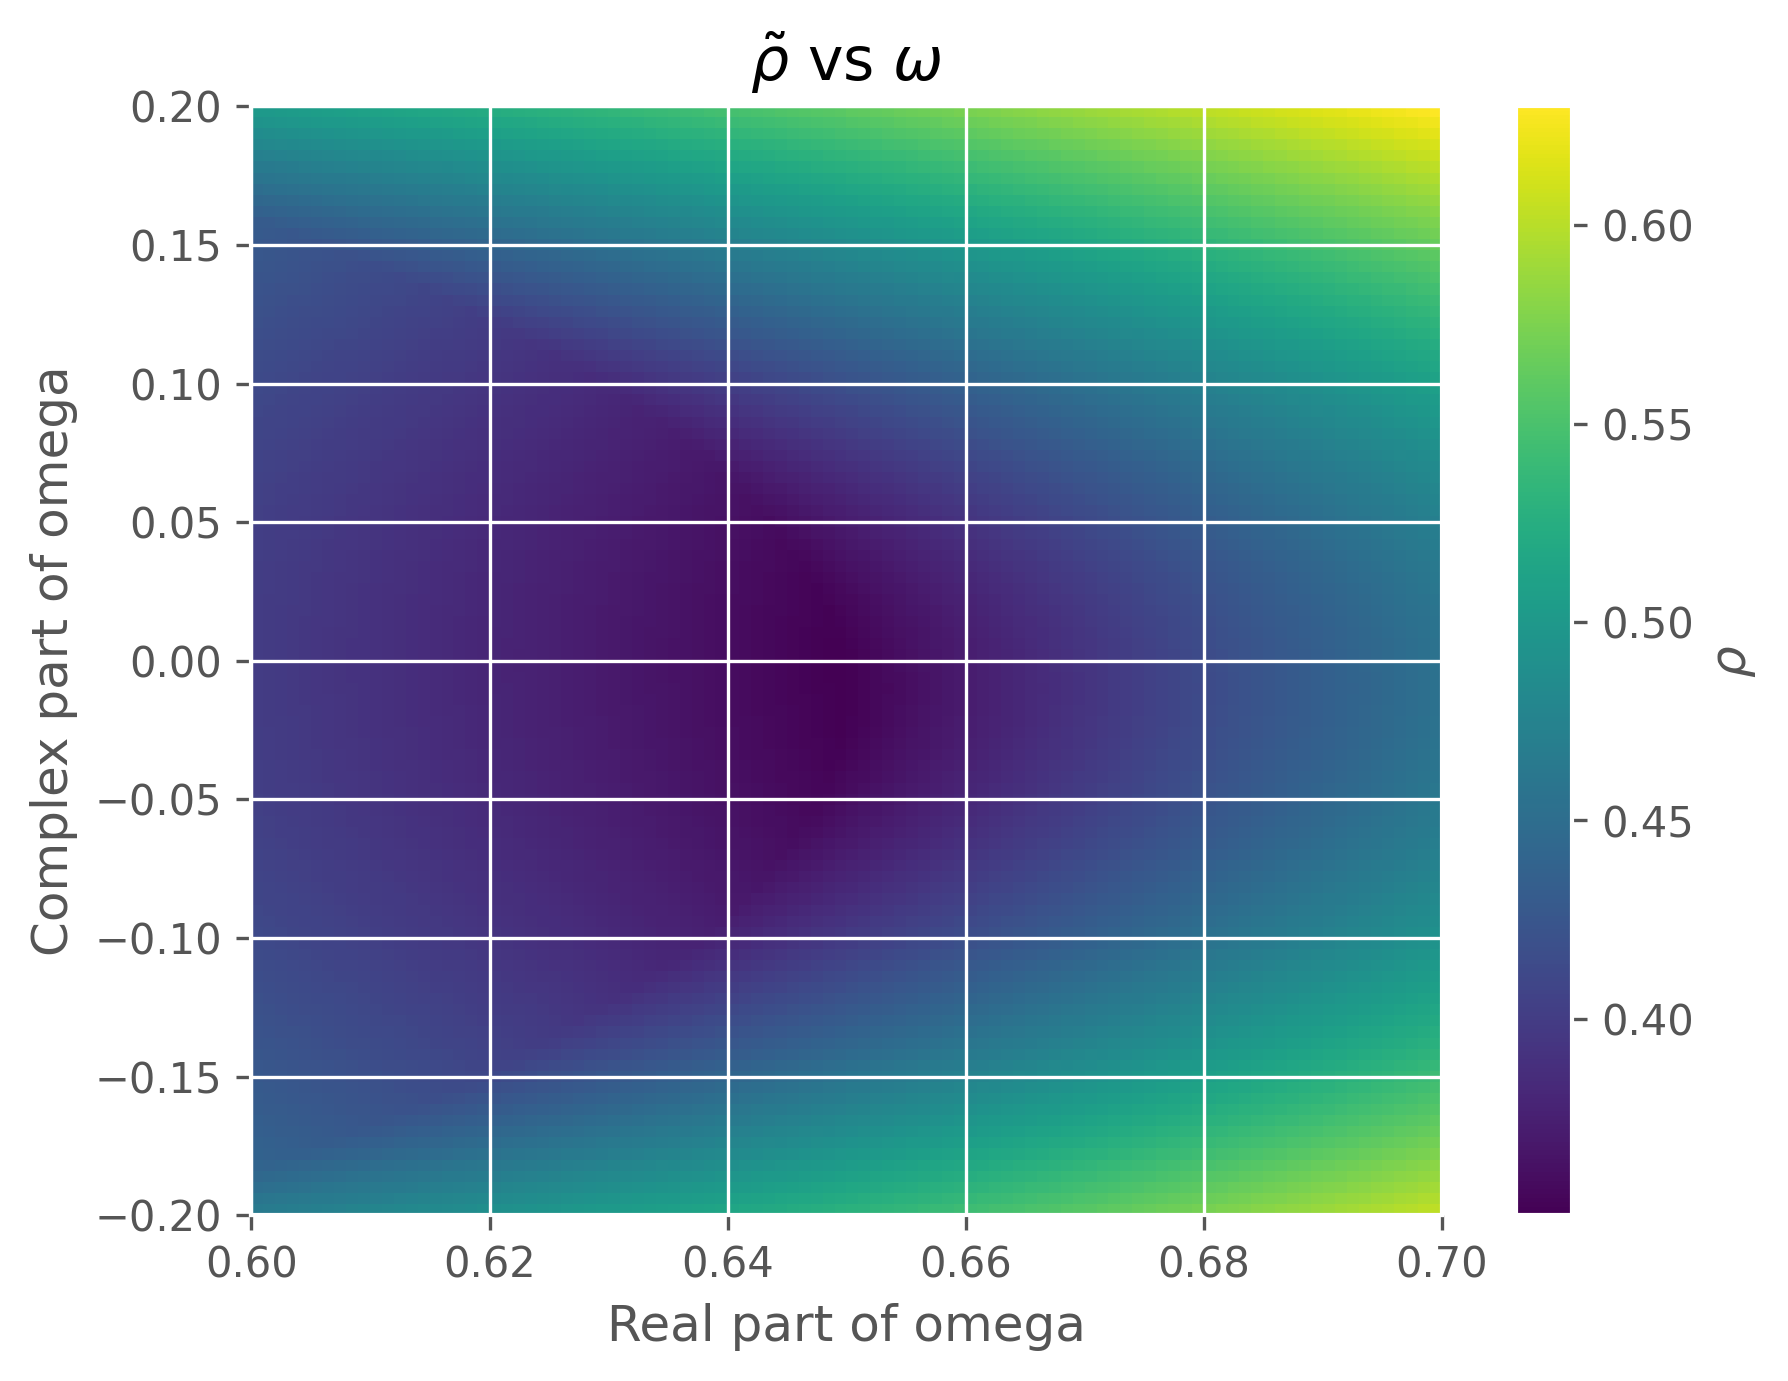
\includegraphics[width=0.8\textwidth]{../code/plts/rho_omega_1Dcomplex.png}
    \caption{}
    \label{fig:rho omega 1D complex}
\end{figure}

\subsection{Spectral analysis of the two-grid correction scheme}
(a) \\
See Figure \ref{fig:rho k complex G}. We used the formula not numerical eigenvalues ... \\
\begin{figure}[h!]
    \centering
    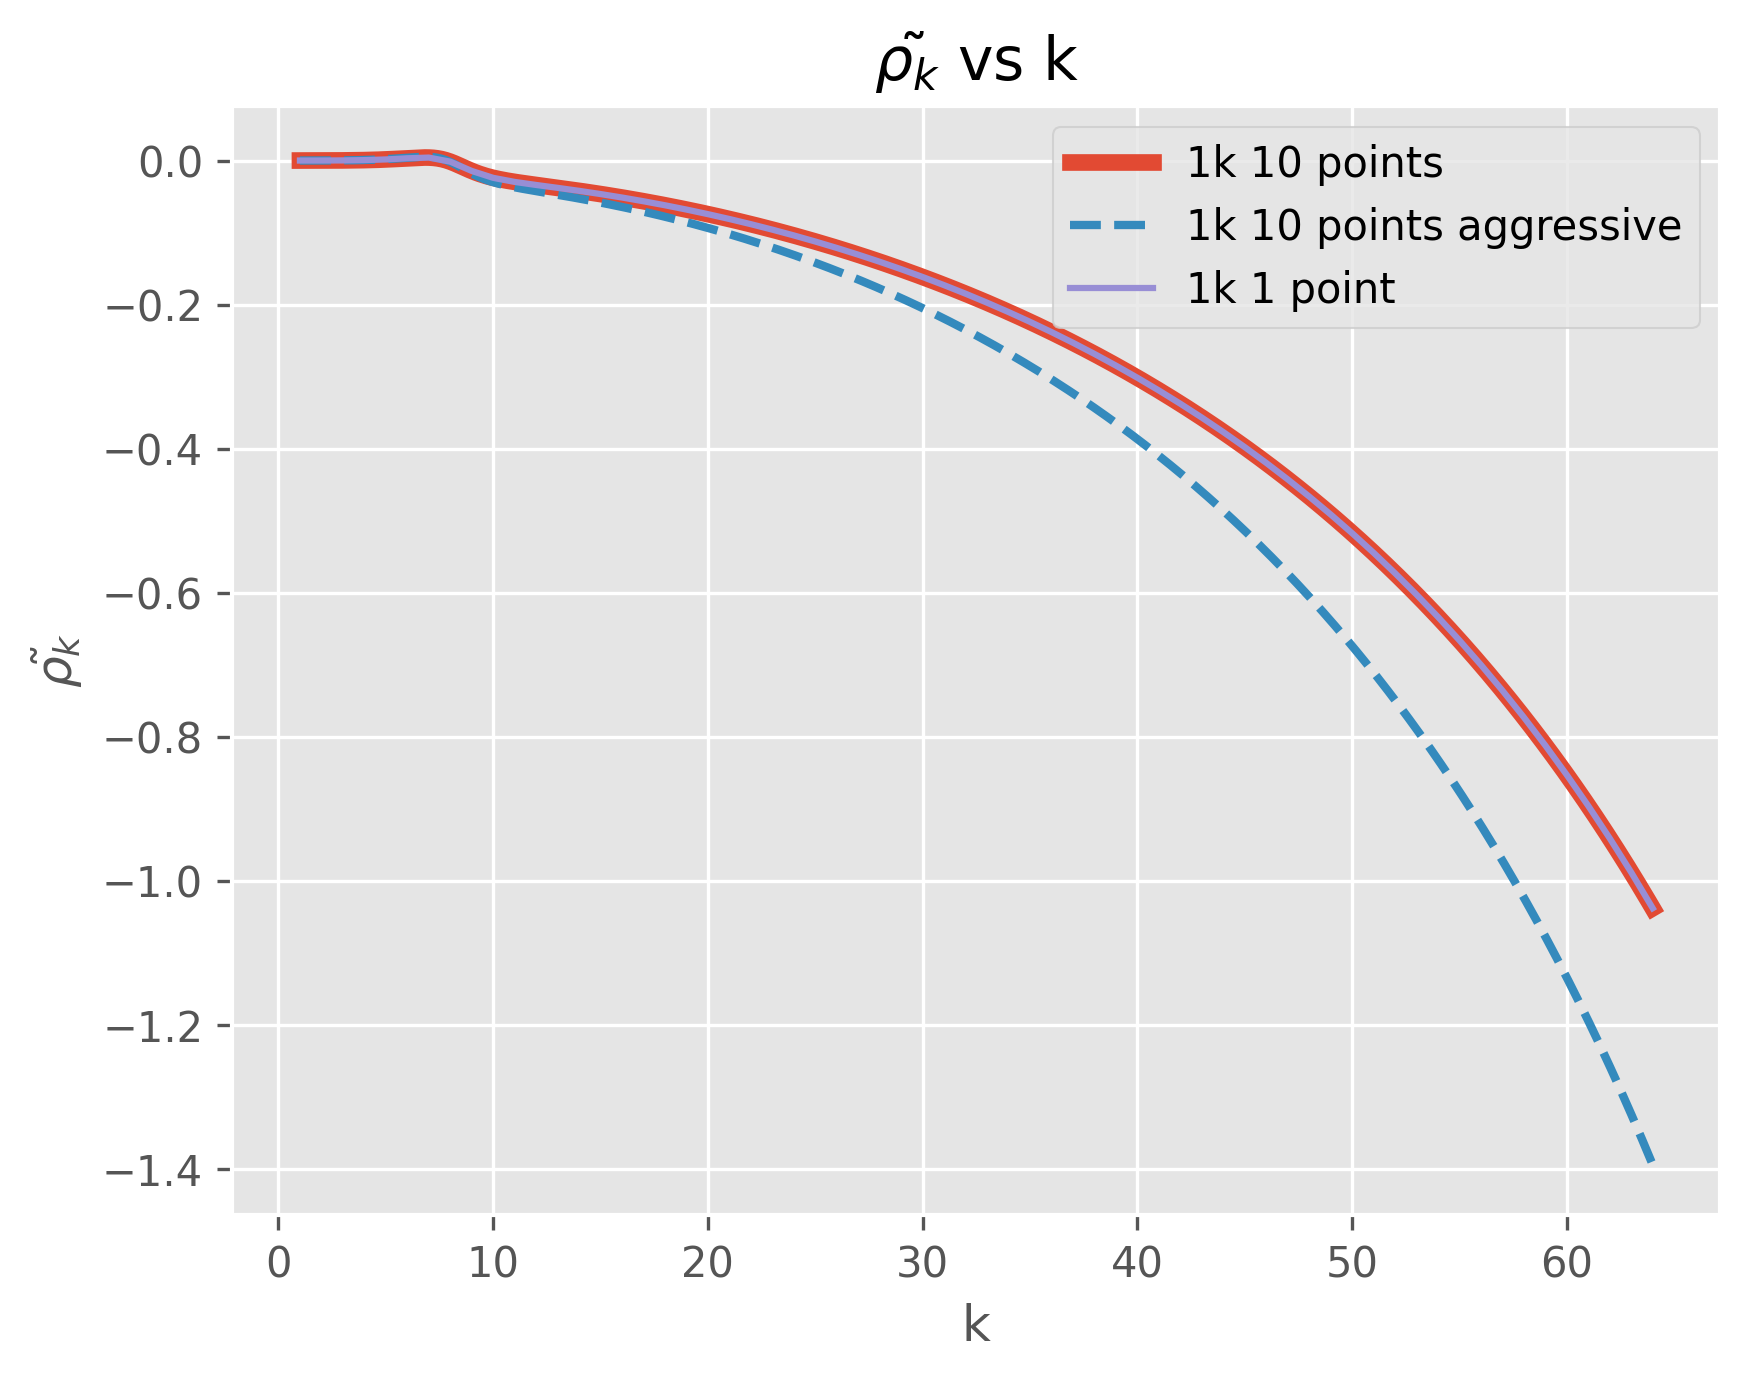
\includegraphics[width=0.8\textwidth]{../code/plts/rho_k_1DcomplexG.png}
    \caption{}
    \label{fig:rho k complex G}
\end{figure}

(b) \\
The instability in $\rho_{k}$ dampens. Compare
\[
    \frac{\varepsilon + \beta j}{ \tilde{\varepsilon} + \beta j }
    \text{ vs }
    \frac{-\varepsilon + \beta j}{ \tilde{\varepsilon} + \beta j  }
    .\]
with $\varepsilon$ small, if $\beta = 0$, these are constants with different signs, for big enough
$\beta$ they are both roughly $1$.

\subsection{2D model problem}
(a) \\
\begin{figure}[h!]
    \centering
    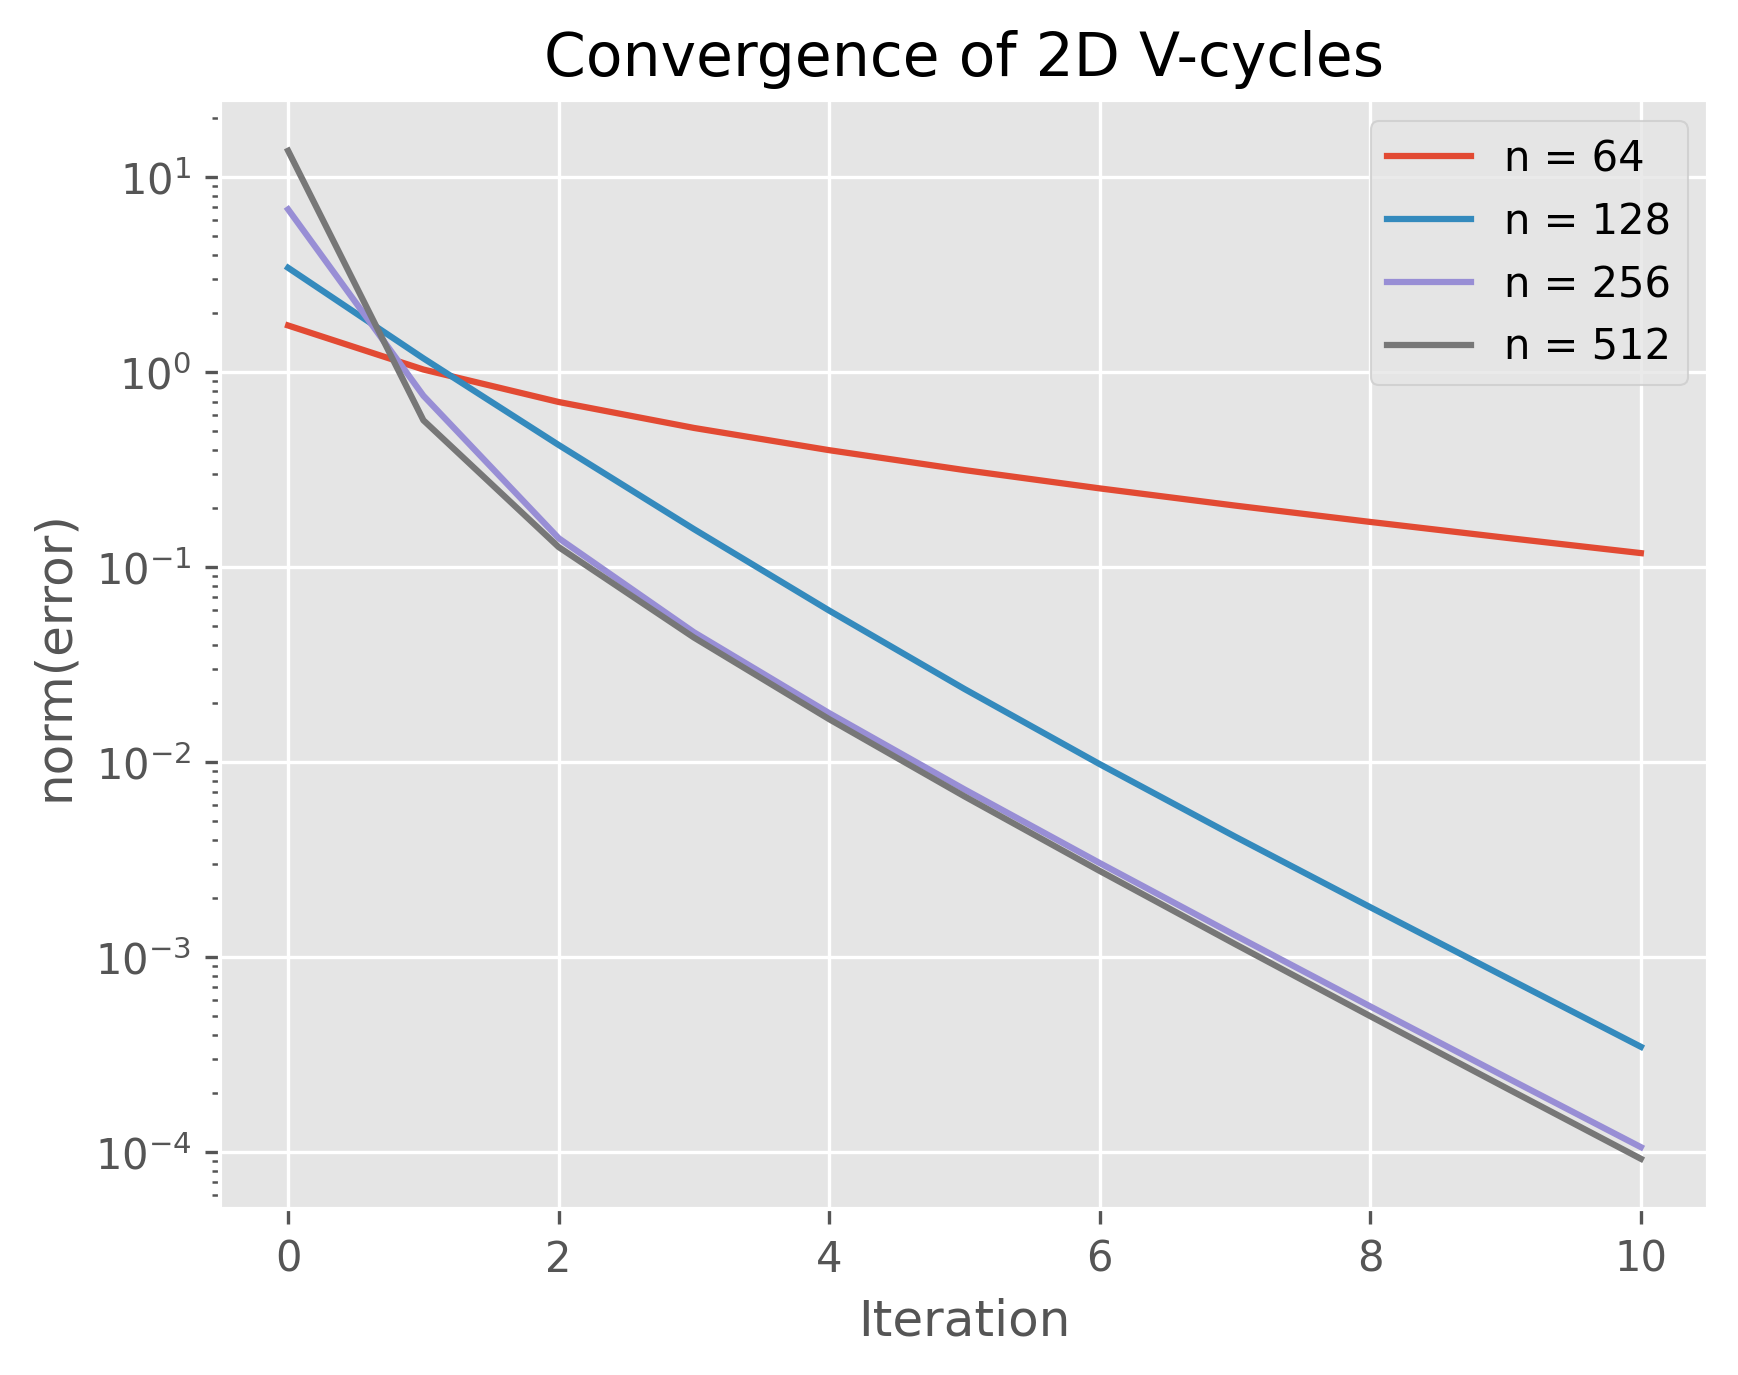
\includegraphics[width=0.8\textwidth]{../code/plts/convergence_2Dcomplex.png}
    \caption{
        Convergence behavior of the V-cycles for solving
        the discretized Helmholtz equation in 2D with $\sigma = -600-300j$ and different $n$.
    }
    \label{fig: convergence 2D complex}
\end{figure}

(b) \\
Less iterations are needed for the same amount of error. This is because
$\sigma$ the source of the problem get relatively smaller to $n^{2}$ in
our convergence factors, asymptotically behavior should go back the
Laplace problem.

\subsection{Aggressive coarsening}
(a)\\
Not sure here is our guess: (TG = two grid,FG = four grid)
\begin{equation}
    FG = I -P_{2n} P_{n} H_{n}^{-1} R_{2n} R_{4n} H_{4n}.
\end{equation}
Not sure what is meant by the eigenmode analysis but what we previously
did does generalizes. The eigenmodes that are complementary with $w_{k}^{4n}$ on
the $n$ grid are: $w_{4n-k}^{4n},w_{2n-k}^{4n},w_{2n+k}^{4n}$. \\
(b)\\
Our solver diverged. Basically we are skipping a smoothing step which
makes the interpolation worse. Also relevant is that convergence
for this problem is better on larger grids. In the FG eigenmode analysis, interpolation error is worse
and eigenvalues are less similar which suggest that only the smoothest modes of the errors get dampend.
Accuracy drops but the trade off is that aggressive coarsening is less expensive about $\frac{1}{2^{d}}$
cheaper on everything but the operations on the base grid. (Half the geometric series is gone.)

\section{Multigrid as a preconditioner for Krylov subspace methods}

\subsection{MG-GMRES for the indefinite Helmholtz problem}
(a) \\
(b) \\
(c) \\
We tried different $\beta$. It seems that to small $\beta$ suffers from the instability problem and
to big $\beta$ would make the problem to different to use to precondition.

\end{document}

% Base your answers on the report.  
% You are expert in giving and revising homework.
%
% Answer as a markdown file.
% Use subnumerings in mark down form in numbering the question 
% that works in a markdown file and use different headers. Like this: 
%
% #  1. Question?
% answer
%
% Here are the questions : 
% 1. Are all requirements of the project met?
% 2. Are there any writing errors?
% 3. What are the most unclear parts in the report?
% 4. Suggest improvements. 
% 5. Are all letter (letter) "entered" properly?